\chapter{Cubed-sphere finite-volume methods}
\label{chp-cs-fv}
In this chapter, we demonstrate the application of the dimension splitting method,
presented in Chapter \ref{chp-2d-fv}, to solve the advection equation on the cubed-sphere based on \citet{putman:2007}.
One significant difference is that on the cubed-sphere, special attention must be given to the stencils near the cube edges.
Additionally, when employing ghost cell layers, the flux at the cube edges is computed twice,
requiring treatment to ensure a unique value in order to achieve mass conservation.

This chapter is organized as follows: Section \ref{chp-cs-adv} introduces the advection equation on the cubed-sphere.
Section \ref{chp-cs-fvcs} presents its finite-volume discretization with a focus on the extension of dimension splitting (Section \ref{sec-csdsplit}) 
as presented in Section \ref{sec-dsplit}.
Numerical experiments are presented in Section \ref{chp-cs-numexpadv}, where we use dimension splitting to assess its
accuracy in computing the divergence of a given vector field to check its numerical consistency, as well as to solve the advection equation.
In particular, we explore different treatments for the cube edges. Section \ref{chp-cs-conc} presents the final thoughts.

\section{Cubed-sphere advection equation in integral form}
\label{chp-cs-adv}
Given a tangent velocity field $\boldsymbol{u}$ on the sphere, we denote its
contravariant components by ${u}$ and ${v}$.
We shall use all the notations introduced in Section \ref{cs-notation}.
The advection equation on panel the $p$ of the cubed-sphere with initial condition $q_0$ is given by:
\begin{equation}
	\begin{cases}
	\label{eq1-adv-cs}
	\bigg[{\partial}_t{q}+
	\frac{1}{\sigma}\bigg(
	{\partial}_x{({u} q \sigma)}+
	{\partial}_y{({v} q \sigma)}
	\bigg)\bigg](x,y,p,t)
	= 0,\\
	q(x,y,p,0) = q_0(x,y,p),
	\end{cases}
\end{equation}
$\forall (x,y) \in [-a,a]^2$, $t\in[0,T]$.
We denote by $\nabla \cdot (q\boldsymbol{u})$ the divergence operator:
\begin{equation}
	\label{advcs:eqdiv}
	\nabla \cdot (q\boldsymbol{u})(x, y, p, t) =  \frac{1}{\sigma}
	[{\partial_x (uq\sigma)} + {\partial_y (vq\sigma)}](x, y, p, t).
\end{equation}
We recall that we say the $\boldsymbol{u}$ is \textbf{non-divergent} if $\nabla \cdot \boldsymbol{u}=0$.
We define the $\mathcal{CS}_N$ grid function $\delta^n$ as
the exact divergence of $q\boldsymbol{u}$ at the cell centers, namely
\begin{equation}
	\label{cs-discrete-div}
	\delta^n_{ijp} = \nabla \cdot (\boldsymbol{u}q)(x_i,y_j,p,t^n).
\end{equation}
Since the metric tensor does not depend on $t$, we may rewrite Equation \eqref{eq1-adv-cs} as
\begin{equation}
	\label{eq2-adv-cs}
	\bigg[{\partial}_t{(q \sigma)}+
	{\partial}_x{({u}q \sigma)}+
	{\partial}_y{({v}q \sigma)}
	\bigg](x,y,p,t)
	= 0.
\end{equation}
Therefore, as in Problem \eqref{chp3-sec2-prob1}, the integral form of Equation \eqref{eq1-adv-cs}
is stated in Problem \eqref{chp5-prob1}.
\begin{prob}
	\label{chp5-prob1}
	Given an initial condition ${q}_0$ and
	a velocity on the sphere $\boldsymbol{u}$, with contravariant components $(u,v)$ on the cubed-sphere coordinate system,
	we would like to find a weak solution ${q}$
	of the cubed-sphere advection equation in its integral form:
	\begin{align*}
		\int_{x_1}^{x_2} \int_{y_1}^{y_2}
		{(q\sigma)}(x, y, p, t) \,dx \,dy = &\int_{x_1}^{x_2} \int_{y_1}^{y_2}
		{(q\sigma)}(x, y, p, t) \,dx \,dy \\ \nonumber
		&-\int_{t_1}^{t_2} \int_{y_1}^{y_2} \bigg({(uq\sigma)}(x_2, y, t)
		-{(uq\sigma)}(x_1, y, t) \bigg) \,dy \,dt\\ \nonumber
		&-\int_{t_1}^{t_2} \int_{x_1}^{x_2} \bigg({(vq\sigma)}(x, y_2, t)
		-{(vq\sigma)}(x, y_1, t) \bigg) \,dx \,dt.
	\end{align*}
	$\forall [x_1, x_2]\times [y_1, y_2] \times[t_1, t_2] \subset \Omega \times[0,T]$, and
	$q(x,y,p,0)=q_0(x,y,p)$.
\end{prob}
Similarly to Section \ref{chp2-sec1}, Equation \eqref{eq1-adv-cs} and Problem \eqref{chp5-prob1} are equivalent
when ${q}, \boldsymbol{u} \in \mathcal{C}^1(\mathbb{S}^2_R)$.
For Problem \ref{chp5-prob1}, the total mass in $\mathbb{S}^2_R$ is defined by: 
\begin{equation}
	{M}_{\mathbb{S}^2_R}(t) = \sum_{p=1}^6 \int_{\Omega} {(q\sigma)}(x,y,p,t) \,dx \,dy , \quad \forall t \in [0,T],
\end{equation}
and is conserved within time: 
\begin{equation}
	{M}_{\mathbb{S}^2_R}(t) = {M}_{\mathbb{S}^2_R}(0), \quad \forall t \in [0,T].
\end{equation}
We define a discretized version of Problem \eqref{chp5-prob1} as Problem \eqref{chp5-prob2}.
\begin{prob}
	\label{chp5-prob2}
	Assume the framework of Problem \ref{chp5-prob1}
	and consider a $(\Delta x, \Delta y, \Delta t, \lambda)$-discretization of $\Omega\times [0,T]$, with $\Delta x= \Delta y$.
	Since we are in the framework of Problem \ref{chp5-prob1}, it follows that:
	\begin{align*}
		{Q}_{ijp}(t_{n+1})  = {Q}_{ijp}(t_{n})
		&- \lambda \frac{\Delta x  \Delta y}{|\Omega_{ijp}|}
		\delta _x \bigg( \frac{1}{\Delta t \Delta y}
		\int_{t^n}^{t^{n+1}} \int_{y_{j-\frac{1}{2}}}^{y_{j+\frac{1}{2}}} 
		{(uq\sigma)}(x_{i}, y, p, t)
		\,dy \,dt \bigg) \\ \nonumber
		&- \lambda \frac{\Delta x  \Delta y}{|\Omega_{ijp}|}
		\delta _y \bigg( \frac{1}{\Delta t \Delta x}
		\int_{t^n}^{t^{n+1}} \int_{x_{i-\frac{1}{2}}}^{x_{i+\frac{1}{2}}} 
		{(vq\sigma)}(x, y_{j}, p, t)
		\,dx \,dt \bigg),
	\end{align*}
	where
	\begin{equation}
	 {Q}_{ijp}(t) = \frac{1}{|\Omega_{ijp}|}
	\int_{x_{i-\frac{1}{2}}}^{x_{i+\frac{1}{2}}} 
	\int_{y_{j-\frac{1}{2}}}^{y_{j+\frac{1}{2}}} {(q\sigma)}(x,y,p,t) \,dx \,dy.
	\end{equation}
	Our problem now consists of finding the values ${Q}_{ijp}(t_{n})$, 
	$\forall i = 1, \ldots, N$, $\forall j = 1, \ldots, M$, $\forall n = 0, \ldots, N_T-1$,
	given the initial values ${Q}_{ijp}(0)$, $\forall i = 1, \ldots N$, $\forall j = 1, \ldots, M$.
	In other words, we aim to find the average values of ${q}$ in each control volume $\Omega_{ijp}$ at the specified time instances.
\end{prob}
It is important to note that no approximations have been made in Problems \eqref{chp5-prob1} and \eqref{chp5-prob2}. 
In practice, the term $\frac{\Delta x  \Delta y}{|\Omega_{ijp}|}$ is estimated using the second-order
formula obtained by applying the midpoint rule in Equation \eqref{chp4-area}:
\begin{equation}
\frac{\Delta x  \Delta y}{|\Omega_{ijp}|}= \frac{1}{\sigma_{ijp}} + O(\Delta x^2).
\end{equation}

\section{Finite-volume on the cubed-sphere approach}
\label{chp-cs-fvcs}
We are ready to introduce the finite-volume scheme on the cubed-sphere (CS-FV).
A CS-FV scheme problem as follows in Problem \ref{chp5-prob3}.
\begin{prob}[CS-FV scheme]
	\label{chp5-prob3}
	Assume the framework defined in Problem \ref{chp5-prob2}.
	The finite-volume approach of Problem \ref{chp5-prob1}
	consists of a finding a scheme of the form:
	\begin{align}
		\label{chp5-csfv}
		{Q}_{ijp}^{n+1} =  {Q}_{ijp}^{n} - \frac{\lambda}{\sigma_{ijp}}\delta_i {F}_{ijp}^{n}
		- \frac{\lambda}{\sigma_{ijp}} \delta_j {G}_{ijp}^{n},
		\\ \nonumber \quad \forall i = 1, \ldots, N, \quad \forall j = 1, \ldots, M, \quad p =1, \ldots, 6,
		\quad \forall n = 0, \ldots, N_T-1,
	\end{align}
	where $ \delta_i F_{ijp}^n =
	{F}_{i+\frac{1}{2},j,p}^{n} 
	- {F}_{i-\frac{1}{2},j,p}^{n}$,
	$ \delta_j G_{ijp}^n =
	{G}_{i,j+\frac{1}{2},p}^{n} 
	- {G}_{i,j-\frac{1}{2},p}^{n}$ 
	and ${Q}^{n}\in \mathcal{CS}_N$ is intended to be an approximation
	of ${Q}(t_{n})\in \mathcal{CS}_N$ in some sense. We define ${Q}_{ijp}^{0} = {Q}_{ijp}(0)$ or
	${Q}_{ijp}^{0} = {q}^0_{ijp}$.
	
	The term ${F}_{i+\frac{1}{2}, j, p}^{n}$ is known as numerical flux in the 
	$x$ direction and it approximates
	$\frac{1}{\Delta t \Delta y}\int_{t_n}^{t_{n+1}} 
	\int_{y_{j-\frac{1}{2}}}^{y_{j+\frac{1}{2}}} 
	(uq\sigma)(x_{i+\frac{1}{2}}, y, p, t) \,dy \,dt $,
	$\forall i = 0, 1, \ldots, N$, and 
	${G}_{i, j+\frac{1}{2}, p}^{n}$ is known as numerical flux in the 
	$y$ direction and it approximates
	$\frac{1}{\Delta t \Delta x}\int_{t_n}^{t_{n+1}}  
	\int_{x_{i-\frac{1}{2}}}^{x_{i+\frac{1}{2}}}
	(vq\sigma)(x, y_{j+\frac{1}{2}}, p, t) \,dx \,dt $,
	$\forall j = 0, 1, \ldots, M$,
	or, in other words, they estimate the time-averaged
	fluxes at the control volume $\Omega_{ijp}$ boundaries.
\end{prob}
\begin{remark}
	For Problem \ref{chp5-prob3}, we define the CFL number in the $x$ and $y$ direction
	by $\max \{{|u_{i+\frac{1}{2},j}^n}|\}\frac{\Delta t}{\Delta x}$ and 
	$\max \{ {|v_{i,j+\frac{1}{2}}^n}|\}\frac{\Delta t}{\Delta y}$, respectively.
	The CFL number is maximum between these numbers and we say that the CFL condition is
	satisfied if the CFL number is less than one. 
\end{remark}
As we mentioned in Problem \ref{chp5-prob3}, the initial condition may be assumed as $q_{ijp}^0$ or $Q_{ijp}(0)$.
We are going to assume  $q_{ijp}^0$ as initial data to avoid the computation of integrals.
Furthermore, the errors will be calculated using the values $q_{ijp}^n$ instead of $Q_{ijp}(t_n)$.
As in Section \ref{sec:fv-2d} this approximation leads to a second-order error.

As in Section \ref{sec:fv-2d}  we introduce the notion of discrete divergence,
which allow us to check the consistency of CS-FV schemes.
\begin{definition}[Discrete divergence]
	\label{chp5-def-div}
	For Problem \ref{chp5-prob3}, we define the discrete divergence as a 
	$\mathcal{CS}_N$-grid function $\mathbb{D}^n(Q^n,u^n,v^n)$
	given by:
	\begin{equation}
		\label{chp5-def-div-eq}
		\mathbb{D}_{ijp}^n(Q^n,u^n,v^n)=  \frac{1}{\Delta t \sigma_{ijp}}
		\bigg(\frac{\delta_i {F}_{ijp}^{n}}{\Delta x} + \frac{\delta_j {G}_{ijp}^{n}}{\Delta y} \bigg), 
		\quad i = 1, \ldots, N, \quad j=1, \ldots,M.
	\end{equation}
\end{definition}
With the aid of the discrete divergence, Equation \eqref{chp5-csfv} becomes:
	\begin{equation}
	\label{chp5-def-div-eq2}
	Q^{n+1} = Q^n - \Delta t \mathbb{D}^n(Q^n,u^n,v^n).
\end{equation}
For a CS-FV scheme the discrete total mass at the time-step $n$ is given by
\begin{equation*}
	M^n =\sum_{p=1}^6 \sum_{i,j=1}^N Q_{ijp}^n \sigma_{ijp} \Delta x \Delta y 
\end{equation*}
It follows from Equation \eqref{chp5-def-div-eq2} that:
\begin{align*}
	M^{n+1} &= M^n  - \sum_{p=1}^6 \sum_{i,j=1}^N \mathbb{D}_{ijp}^{n} \sigma_{ijp} \Delta x \Delta y .
\end{align*}
Hence, to ensure mass conservation, we must ensure that
\begin{align*}
	\sum_{p=1}^6 \sum_{i,j=1}^N   \mathbb{D}_{ijp}^{n} \sigma_{ijp} \Delta x \Delta y = 0.
\end{align*}
This property is discrete version of
\begin{align*}
	\int_{\mathbb{S}^2_R} \nabla \cdot (\boldsymbol{u}q) \,dS = 0,
\end{align*}
which follows from the divergence theorem and the fact of the sphere has no boundary, where $\,dS$ is the surface measure of the sphere.

\subsection{Mass fixer}
\label{mf}
When computing the flux, if we ignore the discontinuity in the cubed sphere coordinate system and use values from adjacent panels
(as in the ET-S72 scheme from Chapter \ref{chp-cs-grids}) to compute stencils, we can ensure mass conservation because the
flux at points lying on the cube edge will be the same.
However, if we consider ghost cell layers by extending the gridlines (as in the ET-DG scheme from Chapter \ref{chp-cs-grids}),
the flux is computed twice at points lying on the cube edge.
Therefore, in this case, some modification is needed to ensure mass conservation (Figure \ref{chp5-fluxcube}).
\begin{figure}[!htb]
	\centering
	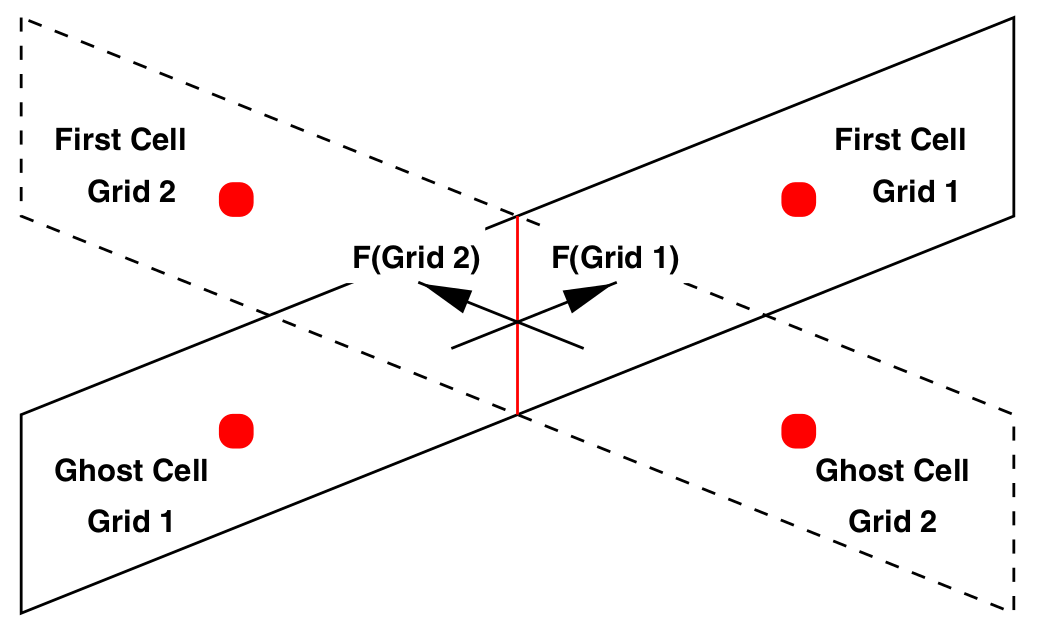
\includegraphics[width=0.5\linewidth]{flux_interface}
	\caption{Figure that illustrates the flux being computed twice on
		the cube edge, breaking the total mass conservation.
		Figure taken from \citet{ross:2006}.\label{chp5-fluxcube}}
\end{figure}

\subsubsection{Average flux at cube interfaces}
\label{mf-av}
One common alternative used in the literature to handle the issue of values being defined twice at points on the
cube edges is to simply average the values (as seen in works such as \citet{ross:2006, chen:2008}).
This approach will be explored in this chapter as one of the mass fixers and is referred to as \textbf{MF-AF}
(AF representing average flux and MF representing mass fixer).

In order to investigate the impact of using the average flux, consider the Figure \ref{chp5-fluxcube} and let us
denote by $Q^n_{1,j,p_1}$ the average value at the first cell on grid 1 and
$Q^n_{N,j,p_2}$ the average value at the first cell on grid 2.
Also, we denote the numerical flux functions from grid 1 by $F_{i+\frac{1}{2},j,p_1}$ and $G_{i,j+\frac{1}{2},p_1}$, 
and the fluxes from grid 2 is given by $F_{i+\frac{1}{2},j,p_2}$ and $G_{i,j+\frac{1}{2},p_2}$.
Therefore, the average values depicted in Figure  \ref{chp5-fluxcube} are updated as follows:
\begin{align}
	Q_{1,j,p_1}^{n+1} &= Q_{1,j,p_1}^n - \frac{\Delta t}{\sigma_{1,j,p_1}} \bigg(
	\frac{F_{1+\frac{1}{2},j,p_1}-F_{\frac{1}{2},j,p_1}}{\Delta x}+
	 \frac{G_{1,j+\frac{1}{2},p_1}-G_{1,j-\frac{1}{2},p_1}}{\Delta y} \bigg), \label{mf-av-eq1}\\
	Q_{N,j,p_2}^{n+1} &= Q_{N,j,p_2}^n - \frac{\Delta t}{\sigma_{N,j,p_2}} \bigg(
	\frac{F_{N+\frac{1}{2},j,p_2}-F_{N-\frac{1}{2},j,p_2}}{\Delta x}+
	\frac{G_{N,j+\frac{1}{2},p_2}-G_{N,j-\frac{1}{2},p_2}}{\Delta y} \bigg).
\end{align}
We also shall assume the following regarding the numerical fluxes consistency:
\begin{align*}
	F_{i+\frac{1}{2},j,p} = \frac{1}{\Delta t \Delta x}
	\int_{y_{j-\frac{1}{2}}}^{y_{j+\frac{1}{2}}} \int_{t^n}^{t^{n+1}} u\sigma q (x_{i+\frac{1}{2}},y,p,t)\,dt \,dy + O(\Delta x^P),\\
	G_{i,j+\frac{1}{2},j,p} = \frac{1}{\Delta t \Delta y}
	\int_{x_{i-\frac{1}{2}}}^{x_{i+\frac{1}{2}}} \int_{t^n}^{t^{n+1}} v\sigma q (x,y_{j+\frac{1}{2}},p,t)\,dt \,dx + O(\Delta x^P),\\
\end{align*}
for any panel $p$.
That is, they are consistent with order $P$.
In particular, at the cube interfaces, we have:
\begin{equation}
\label{mf-av-order}
F_{N+\frac{1}{2},j,p_2}-F_{\frac{1}{2},j,p_1} = O(\Delta x^P).
\end{equation}
The average flux at the cube interface is denoted by:
\begin{equation}
 F^{*}_{\frac{1}{2},j,p_1} = \frac{F_{\frac{1}{2},j,p_1}+F_{N+\frac{1}{2},j,p_2}}{2}.
\end{equation}
Then, if we replace $F^{*}_{\frac{1}{2},j,p_1}$ by $F_{\frac{1}{2},j,p_1}$ in Equation \eqref{mf-av-eq1}, we obtain:
\begin{align*}
	Q_{1,j,p_1}^{n+1} &= Q_{1,j,p_1}^n - \frac{\Delta t}{\sigma_{1,j,p_1}} \bigg(
    \frac{F_{1+\frac{1}{2},j,p_1}-F_{\frac{1}{2},j,p_1}^*}{\Delta x}+
    \frac{G_{1,j+\frac{1}{2},p_1}-G_{1,j-\frac{1}{2},p_1}}{\Delta y} \bigg)\\
	&= 
	Q_{1,j,p_1}^n - \frac{\Delta t}{\sigma_{1,j,p_1}} \bigg(
	\frac{F_{1+\frac{1}{2},j,p_1}-F_{\frac{1}{2},j,p_1}}{\Delta x}+
	\frac{G_{1,j+\frac{1}{2},p_1}-G_{1,j-\frac{1}{2},p_1}}{\Delta y} \bigg)
	+\frac{\Delta t}{\sigma_{1,j,p_1}} 
\frac{(F_{\frac{1}{2},j,p_1}-F_{N+\frac{1}{2},j,p_2})}{2\Delta x}
\end{align*}
Therefore, it follows from Equation \eqref{mf-av-order} that:
\begin{align*}
	\frac{\sigma_{1,j,p_1} \big(Q_{1,j,p_1}^{n+1}- Q_{1,j,p_1}^n\big)}{\Delta t} +
	\bigg(
	\frac{F_{1+\frac{1}{2},j,p_1}-F_{\frac{1}{2},j,p_1}}{\Delta x}+
	\frac{G_{1,j+\frac{1}{2},p_1}-G_{1,j-\frac{1}{2},p_1}}{\Delta y} \bigg)
	= O(\Delta x^{P-1}).
\end{align*}
Hence, the average flux reduces the local truncation
error order by one at the cube interfaces and we expect higher errors at this region.
In particular, if $P=1$, the local truncation error does not converge to zero.
\subsubsection{Divergence projection}
\label{mf-pr}
Another alternative approach, based on Semi-Lagrangian mass corrections
(for a review of these methods, we refer to \citet{diamantakis:2014}),
involves computing the orthogonal projection of the grid function $\mathbb{D}^n$ onto the following space:
\begin{equation*}
	V_0 = \{ \delta \in \mathcal{CS}_N: \quad
		\sum_{p=1}^6 \sum_{i,j=1}^N \mathbb{\delta}_{ijp} \sigma_{ijp} \Delta x \Delta y = 0\},
\end{equation*}
where $V_0$ represents the space of functions with a zero average.
The element of $V_0$ that minimizes its distance to $\mathbb{D}^n$ in the norm 2 is given by:
\begin{equation}
\label{dcor-eq1}
\mathbb{D}^{cor,n}_{ijp} = \mathbb{D}^n_{ijp} - \bigg(\frac{	\sum_{l=1}^6 \sum_{k,m=1}^N \mathbb{D}_{kml}^n \sigma_{kml} \Delta x \Delta y}
 {\sum_{l=1}^6 \sum_{k,m=1}^N \sigma_{kml}^2 \Delta x \Delta y}\bigg)\sigma_{ijp}.
\end{equation}
When employing the projection scheme, we refer to it as \textbf{MF-PR} (PR representing projection).

Our aim now is to investigate the accuracy of this scheme.
Let us assume that the initial divergence approximates the exact divergence with $P$ order
of accuracy, that is
\begin{equation}
\label{dcor-eq2}
	\mathbb{D}^n_{ijp} - \mathbb{\delta}^n_{ijp} = O(\Delta x^P).
\end{equation}
We are interested in giving some bound to 
$\mathbb{D}^{cor,n}_{ijp} - \mathbb{\delta}^n_{ijp}$.
From Equations \eqref{dcor-eq1} and \eqref{dcor-eq2}, it follows that
\begin{equation}
	\label{dcor-eq3}
	\mathbb{D}^{cor,n}_{ijp} - \mathbb{\delta}^n_{ijp} =
	O(\Delta x^P) +  
\bigg( \frac{\sum_{l=1}^6 \sum_{k,m=1}^N \mathbb{D}_{kml}^n \sigma_{kml} \Delta x \Delta y}
{\sum_{l=1}^6 \sum_{k,m=1}^N \sigma_{kml}^2 \Delta x \Delta y}\bigg)\sigma_{ijp}. 
\end{equation}
Hence, it remains to estimate the expression
\begin{equation}
	\label{dcor-eq4}
	\bigg( \frac{\sum_{l=1}^6 \sum_{k,m=1}^N \mathbb{D}_{kml}^n \sigma_{kml} \Delta x \Delta y}
	{\sum_{l=1}^6 \sum_{k,m=1}^N \sigma_{kml}^2 \Delta x \Delta y}\bigg)\sigma_{ijp}.
\end{equation}
From the midpoint rule (Corollary \ref{anexo-mdp-2d}), we have
\begin{align}
	\sum_{l=1}^6 \sum_{k,m=1}^N	\mathbb \sigma_{kml}^2 {\Delta x \Delta y}  &= 
	\sum_{l=1}^6 \sum_{k,m=1}^N
	\int_{x_{i-{\frac{1}{2}}}}^{x_{i+{\frac{1}{2}}}}
	\int_{y_{j-{\frac{1}{2}}}}^{y_{j+{\frac{1}{2}}}}
	\sigma^2(x,y,l) \,dx \,dy
	+C_1\Delta x^2,
\label{dcor-eq5}
\end{align}
where $C_1$ is a constant depending on the second derivatives of $\sigma^2$.

Using the divergence theorem we have
\begin{align*}
	\sum_{l=1}^6 \sum_{k,m=1}^N
	\int_{x_{i-{\frac{1}{2}}}}^{x_{i+{\frac{1}{2}}}}
	\int_{y_{j-{\frac{1}{2}}}}^{y_{j+{\frac{1}{2}}}}
	\nabla \cdot (\boldsymbol{u} q)(x,y,l,t^n) \,dx \,dy
	= \int_{\mathbb{S}_R} 	\nabla \cdot (\boldsymbol{u} q) \,dS = 0.\\
\end{align*}
With this equality, applying again the midpoint rule and Equation \eqref{dcor-eq2}, one gets:
\begin{align}
	\sum_{l=1}^6 \sum_{k,m=1}^N
	\mathbb{D}_{kml}^n \sigma_{kml} {\Delta x \Delta y}  &= 
	\sum_{l=1}^6 \sum_{k,m=1}^N
	\mathbb{\delta }_{kml}^n \sigma_{kml}{\Delta x \Delta y} 
	+ {\Delta x \Delta y} \sum_{l=1}^6 \sum_{k,m=1}^N O(\Delta x^P)\sigma_{kml} \nonumber\\
	&= 
	\sum_{l=1}^6 \sum_{k,m=1}^N
	\int_{x_{i-{\frac{1}{2}}}}^{x_{i+{\frac{1}{2}}}}
	\int_{y_{j-{\frac{1}{2}}}}^{y_{j+{\frac{1}{2}}}}
	\nabla \cdot (\boldsymbol{u} q) (x,y,l,t^n) \,dx \,dy
	+C_2\Delta x^2 	+ {\Delta x \Delta y} \sum_{l=1}^6 \sum_{k,m=1}^N O(\Delta x^P)\sigma_{kml}\nonumber \\
	&= C_2\Delta x^2 + {\Delta x \Delta y} \sum_{l=1}^6 \sum_{k,m=1}^N O(\Delta x^P)\sigma_{kml} \nonumber \\
	&= O(\Delta x^2) +  O(\Delta x^P). \label{dcor-eq6}
\end{align}
Finally, by using Equations \eqref{dcor-eq5} and \eqref{dcor-eq6} in Equation \eqref{dcor-eq4}, 
we have from Equation \eqref{dcor-eq3} that:
\begin{equation}
	\label{dcor-eq7}
	\mathbb{D}^{cor,n}_{ijp} - \mathbb{\delta}^n_{ijp} =
	O(\Delta x^2) +  O(\Delta x^P),
\end{equation}
from where we conclude that the divergence projection introduces a second-order error.
Since the schemes considered here are second-order accurate in the best situation, we
can ensure that this divergence correction does not affect the scheme's order.
We point out that if $\nabla \cdot (\boldsymbol{u} q)=0$, then the second-order error is removed.

\section{Dimension splitting}
\label{sec-csdsplit}
In this section, we will utilize the operator splitting method described in Section \ref{sec-dsplit} 
to obtain a CS-FV scheme.
We will focus on 1D fluxes, specifically the PPM fluxes introduced in Section \ref{chp2-sec-flux},
denoted as ${F}_{i+\frac{1}{2},j,p}^n$ and ${G}_{i,j+\frac{1}{2},p}^n$.
To facilitate the notation, we introduce the auxiliary grid functions $\mathbf{F}$ and $\mathbf{G}$ belonging to $\mathcal{CS}_{N}$, defined as follows:
\begin{align*}
	\mathbf{F}_{ijp}({Q^n,\tilde{u}^n}) = -{\lambda} \bigg({F}_{i+\frac{1}{2},j,p}^n(Q^n_{\times,j,p},\tilde{u}^n_{i+\frac{1}{2},j,p})-
	{F}_{i-\frac{1}{2},j,p}^n(Q^n_{\times,j,p},\tilde{u}^n_{i-\frac{1}{2},j,p}) \bigg),
\end{align*}
for $i=1, \ldots, N$, $j=-\nu+1, \ldots, N + \nu$, and
\begin{align*}
	\mathbf{G}_{ijp}({Q^n,\tilde{v}^n}) = -{\lambda} \bigg({G}_{i,j+\frac{1}{2},p}^n(Q^n_{i,\times,p},\tilde{v}^n_{i,j+\frac{1}{2},p})-
	{G}_{i,j-\frac{1}{2},p}^n(Q^n_{i,\times,p},\tilde{v}^n_{i,j-\frac{1}{2},p}) \bigg),
\end{align*}
for $i=-\nu+1, \ldots, N + \nu$  $j=1, \ldots, N$.
The terms $\tilde{u}^n_{i+\frac{1}{2},j,p}$ and $\tilde{v}^n_{i,j+\frac{1}{2},p}$ represent the 
time-averaged winds used in the computation of departure points in the $x$ and $y$ directions, respectively. 
These averages are calculated using either RK1 or RK2 from Section \ref{chp2-sec-dp}. 
To facilitate the description of the 1D fluxes ${F}_{i+\frac{1}{2},j,p}^n$ and ${G}_{i,j+\frac{1}{2},p}^n$, 
we introduce the time-averaged CFL numbers defined as follows:
\begin{align*}
	\tilde{c}_{i+\frac{1}{2},j,p}^{x,n} = \tilde{u}_{i+\frac{1}{2},j,p}^{x,n}\frac{\Delta t}{\Delta x},\
	\tilde{c}_{i,j+\frac{1}{2},p}^{y,n} = \tilde{v}_{i,j+\frac{1}{2},p}^{y,n}\frac{\Delta t}{\Delta y}.
\end{align*}
The discrete divergence is then obtained as:
\begin{equation}
	\label{eqdiv-split}
	\mathbb{D}^n_{ijp} = -\frac{1}{\Delta t \sigma_{ijp}}
	\bigg[
	\mathbf{F}_{ijp}\bigg(Q^n + \frac{1}{2}\mathbf{g}(Q^n,\tilde{v}^n), \tilde{u}^n \bigg) 
	+\mathbf{G}_{ijp}\bigg(Q^n + \frac{1}{2}\mathbf{f}(Q^n,\tilde{u}^n), \tilde{v}^n \bigg) \bigg],
\end{equation}
where the inner advective operators $\mathbf{f}$ and $\mathbf{g}$ are given in Table \ref{chp3-tab1}.

Now, our objective is to describe the 1D fluxes ${F}_{i+\frac{1}{2},j,p}^n$ and ${G}_{i,j+\frac{1}{2},p}^n$. 
It is important to note that these fluxes depend on the edge treatment, as well as the computation of stencils
and metric tensor treatment, as we will see in the following section.

\subsection{Metric tensor treatment}
\label{mt}
\subsubsection{MT-0}
\label{mt-0}
Let us assume that we are given $Q^n$, with its ghost cells filled using some edge treatment.
When solving Equation \eqref{eq1-adv-cs} in the $x$ direction, we need to reconstruct the function $\psi = q\sigma$.
Then, we have a piecewise-parabolic approximation in the $x$ direction:
\begin{align}
	\label{chp5-ppmx-eq1}
	\begin{cases}
		 \psi_{ijp}^x(x;Q_{\times, j,p}^n) = {\psi}_{L,ijp}^x + \Delta {\psi}_{ijp}^x z_i(x) + {\psi}_{6,ijp}^xz_i(x)(1-z_i(x)), \\
		z_i(x) = \frac{x-x_{i-\frac{1}{2}}}{\Delta x},
		\quad x \in X_i,\\
		\psi_{L,ijp}^x  = q_{R,ijp}^x \sigma_{i-\frac{i}{2},j,p}, \quad
		\psi_{R,ijp}^x  = q_{L,ijp}^x \sigma_{i+\frac{i}{2},j,p}, \\
		q_{L,ijp}^x = q_{i-\frac{i}{2},j,p}^n+ O(\Delta x^2),\quad
		q_{R,ijp}^x = q_{i+\frac{i}{2},j,p}^n+ O(\Delta x^2),\\
		\Delta \psi_{ijp}^x = \psi_{R, ijp}^x - \psi_{L, ijp}^x,\quad
		\psi_{6,ijp}^x = 6\bigg(\sigma_{ijp}Q_{ijp}^n - \frac{(\psi_{L,ijp}^x + \psi_{R,ijp}^x)}{2}\bigg),
	\end{cases}
\end{align}
for $i=1, \ldots, N$, $j=-\nu+1, \ldots, M + \nu$, $p=1,\ldots,6$,
and we also construct a piecewise-parabolic approximation in the $y$ direction:
\begin{align}
	\label{chp5-ppmy-eq2}
	\begin{cases}
		\psi_{ijp}^y(y;Q_{i,\times,p}^n) = \psi_{L,ijp}^y + \Delta \psi_{ijp}^y z_j(y) + \psi_{6,ijp}^yz_j(y)(1-z_j(y)),\\ 
		z_j(y) = \frac{y-y_{j-\frac{1}{2}}}{\Delta y},
		\quad y \in Y_j,\\
		\psi_{L,ijp}^y  = q_{R,ijp}^y \sigma_{i,j-\frac{i}{2},p}, \quad
		\psi_{R,ijp}^y  = q_{L,ijp}^y \sigma_{i,j+\frac{i}{2},p}, \\
		q_{L,ijp}^y = q_{i,j-\frac{1}{2},p}^n+ O(\Delta y^2),\quad
		q_{R,ijp}^y = q_{i,j+\frac{1}{2},p}^n+ O(\Delta y^2),\\
		\Delta \psi_{ijp}^y = q_{R,ijp}^y - q_{L,ijp}^y,\quad 
		\psi_{6,ijp}^y = 6\bigg(\sigma_{ijp}Q_{ijp}^n - \frac{(\psi_{L,ijp}^y + \psi_{R,ijp}^y)}{2}\bigg),
	\end{cases}
\end{align}
for $i=-\nu+1, \ldots, N + \nu$, $j=1, \ldots, M$, $p=1,\ldots,6$.
The values $q_{L,ijp}^x$, $q_{R,ijp}^x$, $q_{L,ijp}^y$, and $q_{R,ijp}^y$ are computed using the PPM stencils
as in Section \ref{cs-recon}. Then, integrating the parabolas with the aid of Equation \eqref{chp-sec-flux:numerical-flux1},
 we may express the fluxes as:
\begin{align}
	\label{chp5-flux-xdir}
	&F_{i+\frac{1}{2},j,p}^n ({Q^n_{\times,j,p},\tilde{u}^n_{i+\frac{1}{2},j,p}}) = 
	\int_{x_{i+\frac{1}{2}}-\tilde{u}_{i+\frac{1}{2},j,p}^n\Delta t}^{x_{i+\frac{1}{2}}}
	{\psi_{ijp}^x(x;Q_{\times, j,p}^n) \,dx} =\\ 
	&\tilde{u}^{n}_{i+\frac{1}{2},j,p} \times
	\begin{cases}
		\psi_{R,ijp}^x +\frac{1}{2}(\psi_{6,i,j}^x - \Delta \psi_{ijp}^x){\tilde{c}_{i+\frac{1}{2},j,p}^{x,n}}
		+\frac{1}{3}{\psi_{6,ijp}^x}(\tilde{c}_{i+\frac{1}{2},j,p}^{x,n})^2,
		\quad &\text{if} \quad \tilde{u}_{i+\frac{1}{2},j,p}^n>0,\\ \nonumber
		\psi_{L,i+1,j,p}^x - \frac{1}{2}(\psi_{6,i+1,j,p}^x + \Delta \psi_{i+1,j,p}^x){\tilde{c}_{i+\frac{1}{2},j,p}^{x,n}}
		-\frac{1}{3}{\psi_{6,i+1,j,p}^x}(\tilde{c}_{i+\frac{1}{2},j,p}^{x,n})^2,
		\quad &\text{if} \quad \tilde{u}_{i+\frac{1}{2},j,p}^n\leq0,\nonumber
	\end{cases}
\end{align}
for $i=0, \ldots, N$, $j=-\nu+1, \ldots, M + \nu$, $p=1,\ldots,6$ and 
\begin{align}
	\label{chp5-flux-ydir}
	&G_{i,j+\frac{1}{2},p}^n ({Q^n_{\times,j,p},\tilde{v}^n_{i,j+\frac{1}{2},p}}) =
	\int_{y_{j+\frac{1}{2}}-\tilde{v}_{i,j+\frac{1}{2},p}^n\Delta t}^{y_{j+\frac{1}{2}}}
	{\psi_{ijp}^y(y;Q_{i,\times, p}^n) \,dy} = \\
	&\tilde{v}^n_{i,j+\frac{1}{2},p}\times
	\begin{cases}
		\psi_{R,ijp}^y +\frac{1}{2}(\psi_{6,ijp}^y - \Delta \psi_{ijp}^y){\tilde{c}_{i,j+\frac{1}{2},p}^{y,n}}
		+\frac{1}{3}{\psi_{6,ijp}^y}(\tilde{c}_{i,j+\frac{1}{2},p}^{y,n})^2,
		\quad &\text{if} \quad \tilde{v}_{i+\frac{1}{2},j,p}^n>0,\\ \nonumber
		\psi_{L,i,j+1,p}^y - \frac{1}{2}(\psi_{6,i,j+1,p}^y + \Delta \psi_{i,j+1,p}^y){\tilde{c}_{i,j+\frac{1}{2},p}^{y,n}}
		-\frac{1}{3}{\psi_{6,i,j+1,p}^y}(\tilde{c}_{i,j+\frac{1}{2},p}^{y,n})^2,
		\quad &\text{if} \quad \tilde{v}_{i,j+\frac{1}{2},p}^n\leq0,\nonumber
	\end{cases}
\end{align}
for $i=-\nu+1, \ldots, N + \nu$, $j=0, \ldots, M$, $p=1,\ldots,6$.
This flux formulation that incorporates the metric tensor in the parabolic approximation
is referred to as \textbf{MT-0} (MT stands for metric tensor).

\subsubsection{MT-PL07}
\label{mt-pl07}
Let us assume again that we are given $Q^n$, with its ghost cells filled using some edge treatment.
Another approach to compute the 1D fluxes, employed in \citet{putman:2007} and \citet{lin:2004},
involves disregarding the metric tensor and constructing a piecewise-parabolic approximation of $q$ in the $x$ direction:
\begin{align}
	\label{chp5-ppmx-eq1-pl07}
	\begin{cases}
		q_{ijp}^x(x;Q_{\times, j,p}^n) = q_{L,ijp}^x + \Delta q_{ijp}^x z_i(x) + q_{6,ijp}^xz_i(x)(1-z_i(x)), \\
		z_i(x) = \frac{x-x_{i-\frac{1}{2}}}{\Delta x},
		\quad x \in X_i,\\
		q_{L,ijp}^x = q_{i-\frac{i}{2},j,p}^n+ O(\Delta x^2),\quad
		q_{R,ijp}^x = q_{i+\frac{i}{2},j,p}^n+ O(\Delta x^2),\\
		\Delta q_{ijp}^x = q_{R,ijp}^x - q_{L,ijp}^x,\quad
		q_{6,ijp}^x = 6\bigg(Q_{ijp}^n - \frac{(q_{L,ijp}^x + q_{R,ijp}^x)}{2}\bigg),
	\end{cases}
\end{align}
for $i=1, \ldots, N$, $j=-\nu+1, \ldots, M+\nu$, $p=1,\ldots,6$ and we also construct a piecewise-parabolic
approximation in the $y$ direction:
\begin{align}
	\label{chp5-ppmy-pl07}
	\begin{cases}
		q_{ijp}^y(y;Q_{i,\times}^n) = q_{L,ijp}^y + \Delta q_{ijp}^y z_j(y) + q_{6,ijp}^yz_j(y)(1-z_j(y)),\\ 
		z_j(y) = \frac{y-y_{j-\frac{1}{2}}}{\Delta y},
		\quad y \in Y_j,\\
		q_{L,ijp}^y = q_{i,j-\frac{1}{2},p}^n+ O(\Delta y^2),\quad
		q_{R,ijp}^y = q_{i,j+\frac{1}{2},p}^n+ O(\Delta y^2),\\
		\Delta q_{ijp}^y = q_{R,ijp}^y - q_{L,ijp}^y,\quad
		q_{6,ijp}^y = 6\bigg(Q_{ijp}^n - \frac{(q_{L,ijp}^y + q_{R,ijp}^y)}{2}\bigg),
	\end{cases}
\end{align}
for $i=-\nu+1, \ldots, N+\nu$, $j=1, \ldots, M$, $p=1,\ldots,6$. Then, we integrate the $\sigma q_{ijp}^x$ and
$\sigma q_{ijp}^x$ assuming that metric tensor is constant on each integration domain, and, with the aid of 
Equation \eqref{chp-sec-flux:numerical-flux1}, we get
\begin{align}
	\label{chp5-flux-xdir--pl07}
	&F_{i+\frac{1}{2},j,p}^n ({Q^n_{\times,j,p},\tilde{u}^n_{i+\frac{1}{2},j,p}}) = 
	\int_{x_{i+\frac{1}{2}}-\tilde{u}_{i+\frac{1}{2},j,p}^n\Delta t}^{x_{i+\frac{1}{2}}}
	{\sigma(x,y_j,p) q_{ijp}^x(x;Q_{\times, j,p}^n) \,dx} = \\
	&{\sigma}_{i+\frac{1}{2},j,p}\tilde{u}^{n}_{i+\frac{1}{2},j,p} \times
	\begin{cases}
		q_{R,ijp}^x +\frac{1}{2}(q_{6,ijp}^x - \Delta q_{ijp}^x){\tilde{c}_{i+\frac{1}{2},j,p}^{x,n}}
		+\frac{1}{3}{q_{6,ijp}^x}(\tilde{c}_{i+\frac{1}{2},j}^{x,n})^2,
		\quad &\text{if} \quad \tilde{u}_{i+\frac{1}{2},j,p}^n>0,\\ \nonumber
		q_{L,i+1,j,p}^x - \frac{1}{2}(q_{6,i+1,j,p}^x + \Delta q_{i+1,j,p}^x){\tilde{c}_{i+\frac{1}{2},j,p}^{x,n}}
		-\frac{1}{3}{q_{6,i+1,j,p}^x}(\tilde{c}_{i+\frac{1}{2},j,p}^{x,n})^2,
		\quad &\text{if} \quad \tilde{u}_{i+\frac{1}{2},j,p}^n\leq0,\nonumber
	\end{cases}
\end{align}
for $i=0, \ldots, N$, $j=-\nu+1, \ldots, M+\nu$, $p=1,\ldots,6$ and 
\begin{align}
	\label{chp5-flux-ydir-pl07}
	&G_{i,j+\frac{1}{2},p}^n ({Q^n_{\times,j,p},\tilde{v}^n_{i,j+\frac{1}{2},p}}) =
	\int_{y_{j+\frac{1}{2}}-\tilde{v}_{i,j+\frac{1}{2},p}^n\Delta t}^{y_{j+\frac{1}{2}}}
	{\sigma(x_i,y,p)q_{ijp}^y(y;Q_{i,\times, p}^n) \,dy} = \\
	&{\sigma}_{i,j+\frac{1}{2},p} \tilde{v}^n_{i,j+\frac{1}{2},p}\times
	\begin{cases}
		q_{R,ijp}^y +\frac{1}{2}(q_{6,ijp}^y - \Delta q_{ijp}^y){\tilde{c}_{i,j+\frac{1}{2},p}^{y,n}}
		+\frac{1}{3}{q_{6,i,j,p}^y}(\tilde{c}_{i,j+\frac{1}{2},p}^{y,n})^2,
		\quad &\text{if} \quad \tilde{v}_{i+\frac{1}{2},j,p}^n>0,\\ \nonumber
		q_{L,i,j+1,p}^y - \frac{1}{2}(q_{6,i,j+1}^y + \Delta q_{i,j+1,p}^y){\tilde{c}_{i,j+\frac{1}{2},p}^{y,n}}
		-\frac{1}{3}{q_{6,i,j+1,p}^y}(\tilde{c}_{i,j+\frac{1}{2},p}^{y,n})^2,
		\quad &\text{if} \quad \tilde{v}_{i,j+\frac{1}{2},p}^n\leq0,\nonumber
	\end{cases}
\end{align}
for $i=-\nu+1, \ldots, N+\nu$, $j=0, \ldots, M$, $p=1,\ldots,6$.
This flux formulation is referred to as \textbf{MT-PL07} and introduces a first-order
error because of the assumption of a constant metric tensor on each integration domain.

\subsection{Flux at edges treatment}
If we choose the ET-DG scheme, we will calculate the required wind values for ghost positions as
described in Section \ref{cs-wind-interp}.
However, this scheme requires modifying the flux at the edges to maintain mass conservation.
To achieve this, we will apply the mass fixer schemes discussed earlier.
Using these flux values, we can compute the discrete divergence (Equation \eqref{eqdiv-split}) for the interior cells and update the solution for the next time step.

On the other hand, if we utilize the ET-PL07 scheme, we will populate the scalar field and velocity field contravariant
components at ghost cell positions with the adjacent panel values, similar to the ET-S72 scheme.
This allows us to compute $\mathbf{F}$ and $\mathbf{G}$ at all necessary positions and we can update the solution.
In the PPM reconstruction, we employ extrapolation near the cubed edges that defines the ET-PL07 scheme.
When combining MT-PL07 with ET-PL07, a first-order error is introduced.
However, we can ensure that the PL07 splitting scheme (Table \ref{chp3-tab1}) eliminates the splitting error when $q$ is constant.

\section{Numerical experiments}
\label{chp-cs-numexpadv}
This section is dedicated to present the numerical experiments for the
advection equation on the sphere. In Table \ref{chp5-tab1} we present
the initial conditions (IC) and in Table \ref{chp5-tab2} we present
the velocity fields (VF) considered.  
\begin{table}[!ht]
	\begin{tabular}{|c|l|l|}
		\hline
		IC name & \multicolumn{1}{c|}{$q_0$} \\ \hline
		IC1   & $\exp(b_0((X-X_0)^2+ (Y-Y_0)^2 + (Z-Z_0)^2))$ \\ \hline
        IC2   & $\exp(b_0[(X-X_1)^2+ (Y-Y_1)^2 + (Z-Z_1)^2] + \exp(b_0[(X-X_2)^2+ (Y-Y_2)^2 + (Z-Z_2)^2])$ \\ \hline
		IC3   & $1+ \cos(\lambda)\cos(\phi)\sin(\alpha) - \sin(\phi)\cos(\alpha)$, \\ \hline
	\end{tabular}
	\caption{Initial conditions considered in the numerical experiments (Figure \ref{chp5-ic}).}
	\label{chp5-tab1} 
\end{table}

\begin{table}[!ht]
	\begin{tabular}{|c|l|l|l|}
		\hline
		VF name & \multicolumn{1}{c|}{$u_\lambda(\lambda,\phi,t) $} & \multicolumn{1}{c|}{$v_\phi(\lambda,\phi,t)$}  & \multicolumn{1}{c|}{$\Delta t^{(0)}$}\\ \hline
		VF1   & $u_0(\cos(\phi)\cos(\alpha) + \sin(\phi)\cos(\lambda)\sin(\alpha))$ 
		& $-u_0\sin(\lambda)\sin(\alpha)$ & 0.025  \\ \hline
		VF2   & $k\sin^2(\lambda_p+\pi)\sin(2\phi)\cos(\frac{\pi t}{T})+\frac{2\pi}{T}\cos\phi$ 
		& $k\sin(2(\lambda_p+\pi))\cos(\phi)\cos(\frac{\pi t}{T})$& 0.0125  \\ \hline
		VF3   & $-k\sin^2(\frac{\lambda+\pi}{2})\sin(2\phi)\cos^2(\phi)\cos(\frac{\pi t}{T}),$ 
		& $\frac{k}{2}\sin(\lambda+\pi)\cos^3(\phi)\cos(\frac{\pi t}{T})$ & 0.00625 \\ \hline
	\end{tabular}
	\caption{Velocity fields considered in the numerical experiments and its initial time step $\Delta t^{(0)}$.}
	\label{chp5-tab2}
\end{table}

In Table \ref{chp5-tab1}, $(X_0,Y_0,Z_0)$, $(X_1,Y_1,Z_1)$ and $(X_2,Y_2,Z_2)$ are the Cartesian coordinates of the latitude-longitude points
$(\lambda_0,\phi_0) = (\frac{\pi}{4},\frac{\pi}{6})$,
$(\lambda_1,\phi_1) = (-\frac{\pi}{6},0)$ and
$(\lambda_2,\phi_2) = ( \frac{\pi}{6},0)$.
IC1 represents a Gaussian hill centered at a cube corner and we set $b_0 = -10$.
IC2 represents two Gaussian hills as suggested by \citet{nair:2010} and we set $b_0 = -5$.
IC3 is based on the steady flow presented in \citet{will:1992} and we adopt $\alpha=-\frac{45\pi}{180}$.
The initial conditions are shown in Figure \ref{chp5-ic}.

For the velocities provided in Table \ref{chp5-tab2}, we adopt the following parameter values:
$u_0 = \frac{2\pi}{5}$, $\alpha=-\frac{45\pi}{180}$, $\lambda_p=\lambda-\frac{2\pi t}{T}$, $T=5$.
In this context, VF1 represents the non-divergent rotated zonal field introduced in \citet{will:1992}.
VF2 corresponds to the non-divergent deformational flow described in \citet{nair:2010},
and VF3 represents the divergent flow also presented in \citet{nair:2010}.
Additionally, VF2 utilizes $k=2$ and VF3 uses $k=1$.
For all velocity fields presented here, the initial condition is equal to the final solution after 5 time units.
Also, we consider the unit sphere.

\begin{figure}[!htb]
	\centering
	\begin{subfigure}{0.3\textwidth}
		\centering
		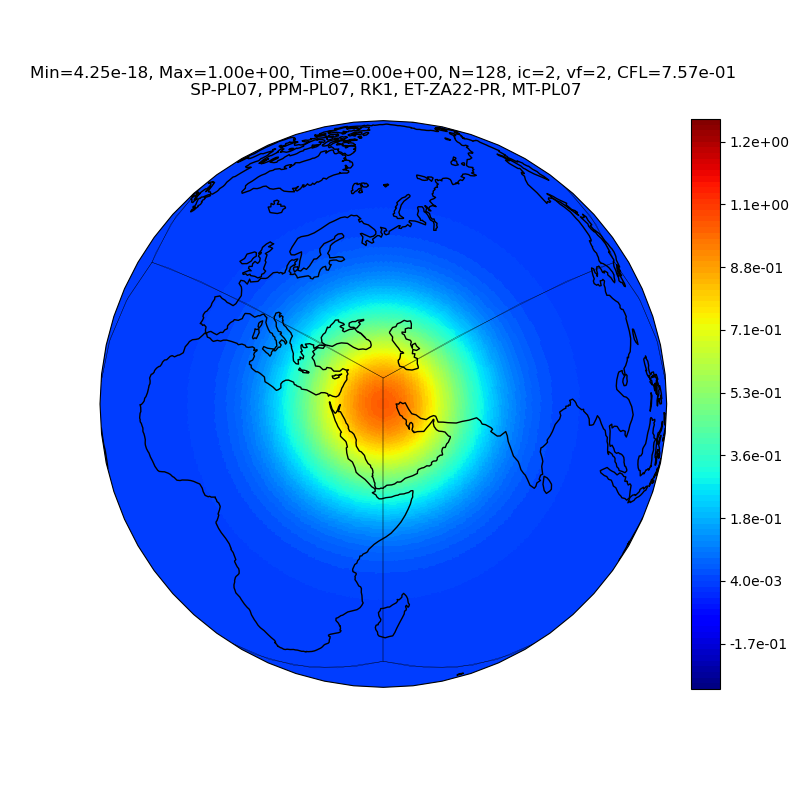
\includegraphics[width=1\linewidth]{gnomonic_equiangular_cs_128_adv_Q_ic2_vf2_SP-PL07_PPM-PL07_RK1_ET-ZA22-PR_MT-PL07_interp3_t0_sphere}
		\caption{IC1. \label{chp5-ic1}}
	\end{subfigure}
	\begin{subfigure}{0.3\textwidth}
		\centering
		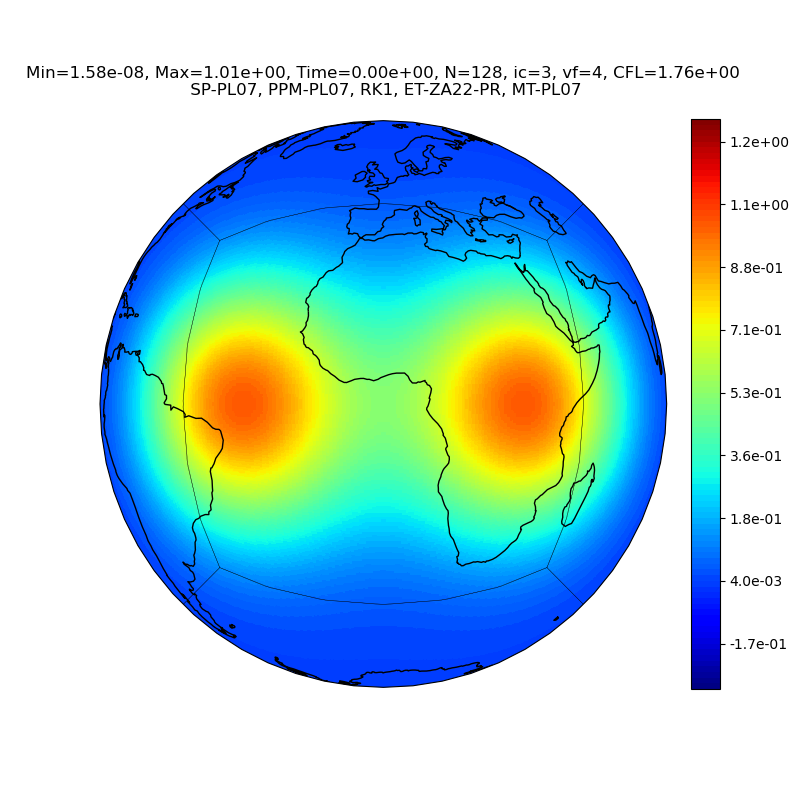
\includegraphics[width=1\linewidth]{gnomonic_equiangular_cs_128_adv_Q_ic3_vf4_SP-PL07_PPM-PL07_RK1_ET-ZA22-PR_MT-PL07_interp3_t0_sphere}
		\caption{IC2. \label{chp5-ic2}}
	\end{subfigure}
	\begin{subfigure}{0.3\textwidth}
		\centering
		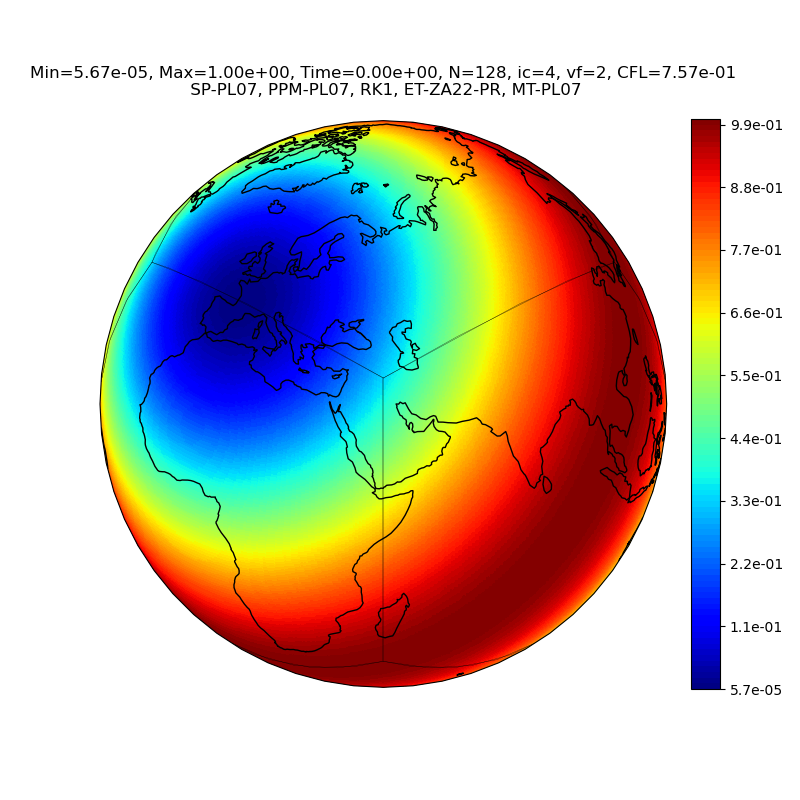
\includegraphics[width=1\linewidth]{gnomonic_equiangular_cs_128_adv_Q_ic4_vf2_SP-PL07_PPM-PL07_RK1_ET-ZA22-PR_MT-PL07_interp3_t0_sphere}
		\caption{IC3. \label{chp5-ic3}}
	\end{subfigure}
	\caption{ Illustration of the initial conditions considered in this chapter (Table \ref{chp5-tab1}) .\label{chp5-ic}}
\end{figure}

To compute the convergence, consider cubed-sphere grids with value of $N_k =  2^{k+4}$,
and $\Delta t^{(k)} = \frac{\Delta t^{(k)}}{2^k}$, $k=0, \ldots, 6$, where
the value of $\Delta t^{(0)}$ in Table \ref{chp5-tab2} for each VF.
The relative error in the maximum norm is computed as
\begin{equation}
	E_k = \frac{\max |Q^{N_T} - Q^0|}{\max {|Q^0|}},
\end{equation}
and the convergence rate is defined as
\begin{equation*}
	CR_k = \frac{\ln{\bigg(\frac{E_{k}}{E_{k-1}}}\bigg)}{\ln 2}, \quad \text{for} \quad k = 1, \ldots 6.
\end{equation*}
In Table \ref{chp5-tab3}, we present all four schemes that we are considering. 
We shall always assume that the PPM-PL07 is employed. 
The main distinction between Scheme 1 and Scheme 2 lies in their ghost cell treatment.
In Scheme 1, we adopt the approach proposed by \citet{putman:2007} for the ghost cell formulation,
while Scheme 2 utilizes the MF-PR scheme.
Both Scheme 1 and Scheme 2 employ the splitting PL07 and the metric tensor formulation MT-PL07 
with the RK1 departure point scheme. On the other hand, Scheme 3 and Scheme 4 utilize the splitting,
the metric tensor formulation MT-0, and the RK2 departure point scheme.
Scheme 1 and Scheme 2 are expected to achieve first-order accuracy, and so is schemes 3, since as we have seen in Section \ref{mf},
the local truncation error when using MF-AF is reduced by one at the cube interfaces.
Scheme 4 is designed
to attain second-order accuracy. Finally, the key difference between Scheme 3 and Scheme 4 lies in the mass fixer.
\begin{table}[!ht]
	\begin{tabular}{|c|l|l|l|l|l|}
		\hline
		Scheme & Splitting & Departure point & Edge Treatment & Mass fixer & Metric tensor\\ \hline
		1   & PL07 & RK1 & ET-PL07 & None & MT-PL07\\ \hline
		2   & PL07 & RK1 & ET-PL07 & None & MT-PL07\\ \hline
		3   & AVLT & RK2 & ET-DG & AF & MT-0\\ \hline
		4   & AVLT & RK2 & ET-DG & PR & MT-0\\ \hline
	\end{tabular}
	\caption{Schemes considered for this Chapter.}
	\label{chp5-tab3} 
\end{table}

\subsection{Divergence of the rotated zonal wind}
For our initial test, we will examine the velocity field VF1, which is non-divergent with $q=1$.
We will calculate its discrete divergence using equation \eqref{eqdiv-split}.
The resulting errors and convergence rates are illustrated in Figure \ref{chp5-error-div}.
\begin{figure}[!htb]
	\centering
	\begin{subfigure}{0.42\textwidth}
		\centering
		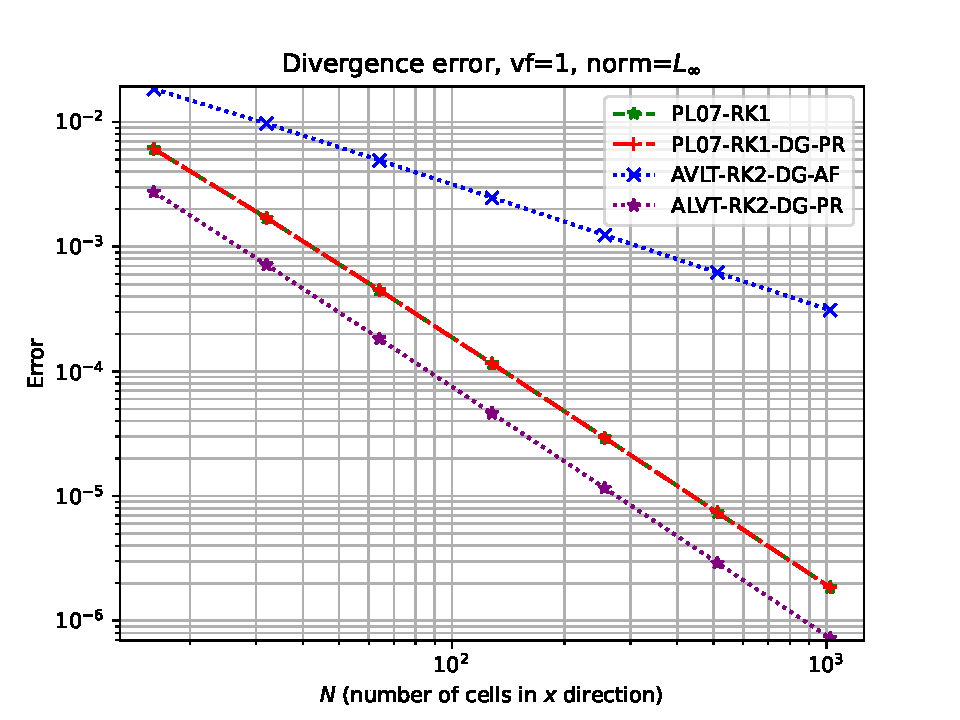
\includegraphics[width=1\linewidth]{cs_div_vf1_normlinf_parabola_errors}
		\caption{Error.\label{chp5-errordiv}}
	\end{subfigure}
	\begin{subfigure}{0.42\textwidth}
		\centering
		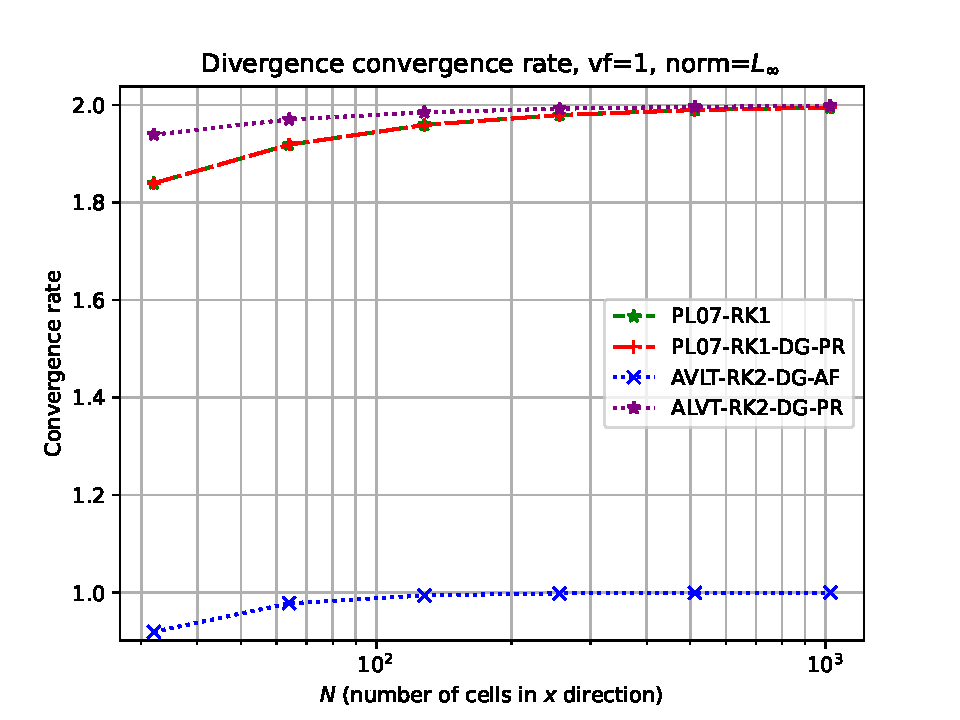
\includegraphics[width=1\linewidth]{cs_div_vf1_normlinf_convergence_rate}
		\caption{Convergence rate.\label{chp5-crdiv}}
	\end{subfigure}
	\caption{Convergence of the error for the schemes from table \ref{chp5-tab3} obtained when computing the divergence of rotated zonal wind VF1.
	\label{chp5-error-div}}
\end{figure}

From the analysis of Figure \ref{chp5-error-div}, we can observe that both Scheme 1 and Scheme 2 yield the same error,
which is of second order. This result aligns with our expectations, as the PL07 splitting scheme possesses the property of eliminating
splitting errors when $q$ is constant, regardless of the edge treatment scheme.
Additionally, we can notice that Scheme 3 exhibits a first-order error, while Scheme 4 demonstrates a second-order error.
Hence, we can conclude that averaging the flux at the cubed edges reduces the scheme's order, while the divergence projection maintains the order.
Examining Figure \ref{chp5-div}, which displays the obtained errors on the sphere, it becomes evident that the averaging
flux introduces a grid-imprinting pattern, wherein the cube edges are observable (see Figure \ref{chp5-div2}).
The Scheme 1,2 and 3 does not present grid-imprinting pattern, but their errors have a strong discontinuity on the panel edges.
\begin{figure}[!htb]
	\centering
	\begin{subfigure}{0.3\textwidth}
		\centering
		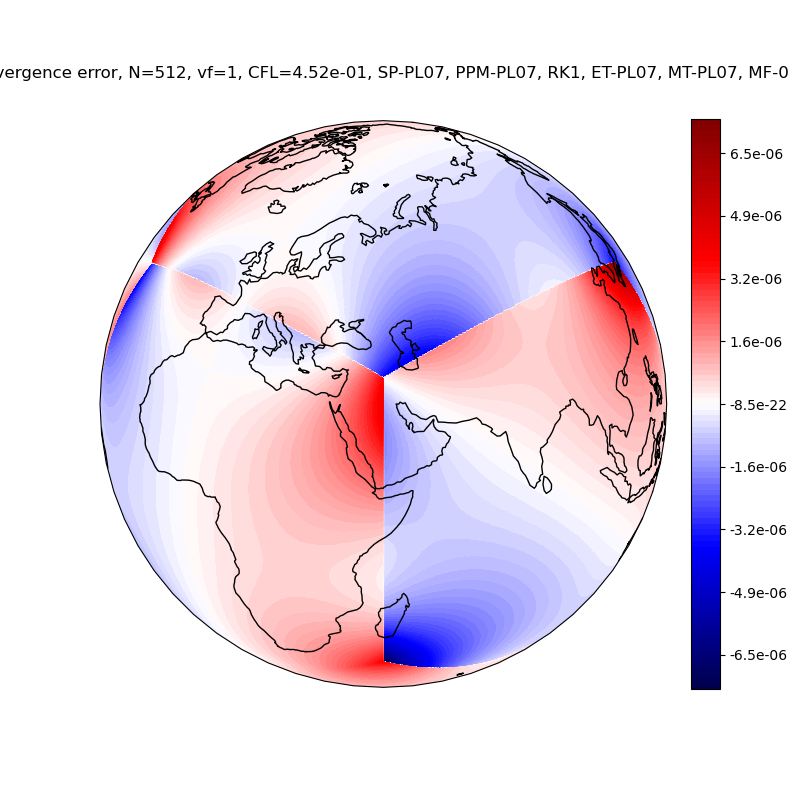
\includegraphics[width=1\linewidth]{gnomonic_equiangular_cs_512_div_error_vf1_SP-PL07_PPM-PL07_RK1_ET-PL07_MT-PL07_MF-0_sphere}
		\caption{Scheme 1 \label{chp5-div1}}
	\end{subfigure}
	\begin{subfigure}{0.3\textwidth}
	\centering
	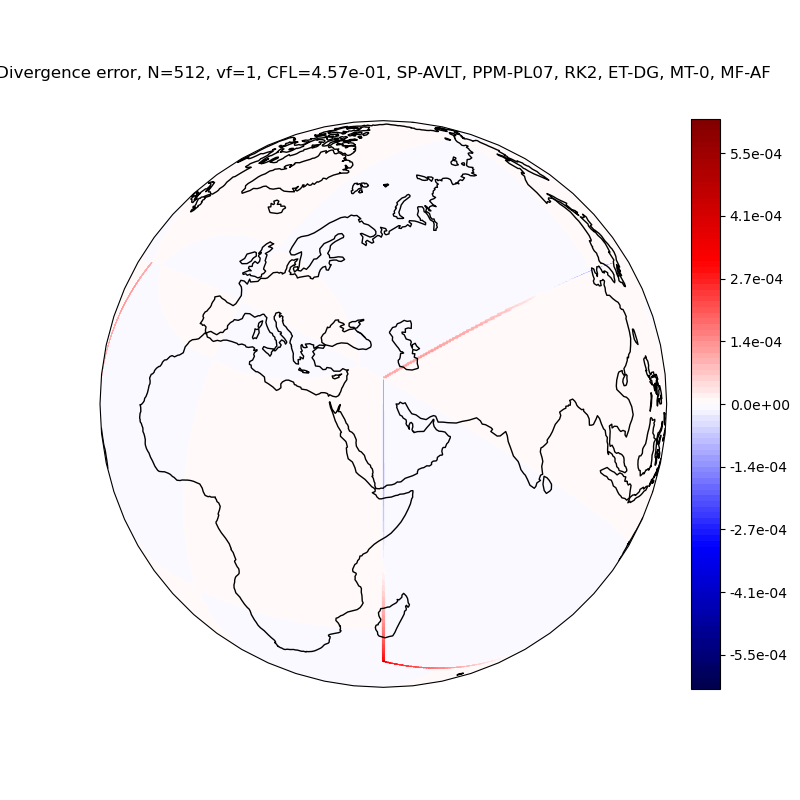
\includegraphics[width=1\linewidth]{gnomonic_equiangular_cs_512_div_error_vf1_SP-AVLT_PPM-PL07_RK2_ET-DG_MT-0_MF-AF_sphere}
	\caption{Scheme 3 \label{chp5-div2}}
	\end{subfigure}
	\begin{subfigure}{0.3\textwidth}
	\centering
	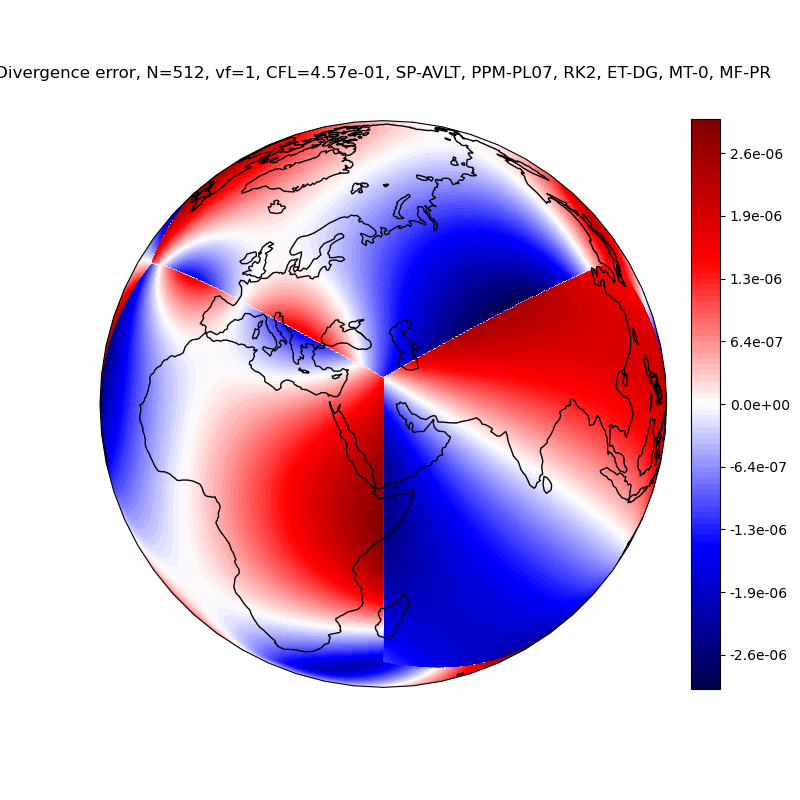
\includegraphics[width=1\linewidth]{gnomonic_equiangular_cs_512_div_error_vf1_SP-AVLT_PPM-PL07_RK2_ET-DG_MT-0_MF-PR_sphere}
	\caption{Scheme 4 \label{chp5-div3}}
	\end{subfigure}
	\caption{ Divergence error obtained for all schemes from table using the VF1 velocity field from table \ref{chp5-tab2}.
		The error of scheme 2 is equal to the error of scheme 1 (Figure 2)
		This figure considers a cubed-sphere with $N=512$. \label{chp5-div}}
\end{figure}

\subsection{Advection of one Gaussian hill through the rotated zonal wind}
As a second test case, we consider the advection of the Gaussian hill given by IC1 using 
the rotated zonal wind VF1.
In Figure \ref{chp5-error-adv1}, we depict the final errors obtained for 
all schemes from Table \ref{chp5-tab2}.
We can observe that schemes 1 and scheme 2 are first-order accurate, while schemes 3 and 4 
are second-order accurate.
Furthermore, it is worth noting that although scheme 3 showed to be only first-order 
accurate in computing the divergence of VF1, the final error after simulating the advection 
equation is second-order accurate.
\begin{figure}[!htb]
	\centering
	\begin{subfigure}{0.4\textwidth}
		\centering
		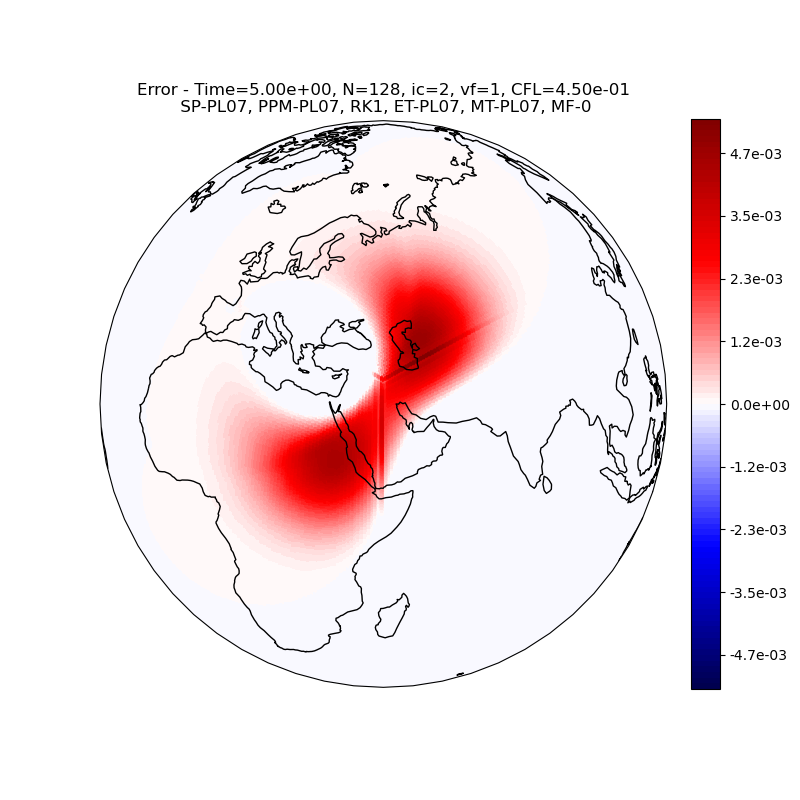
\includegraphics[width=1\linewidth]{gnomonic_equiangular_cs_128_adv_Q_error_ic2_vf1_SP-PL07_PPM-PL07_RK1_ET-PL07_MT-PL07_MF-0_interp3_t1600_sphere}
		\caption{Scheme 1 \label{chp5-adv1-s1}}
	\end{subfigure}
	\begin{subfigure}{0.4\textwidth}
		\centering
		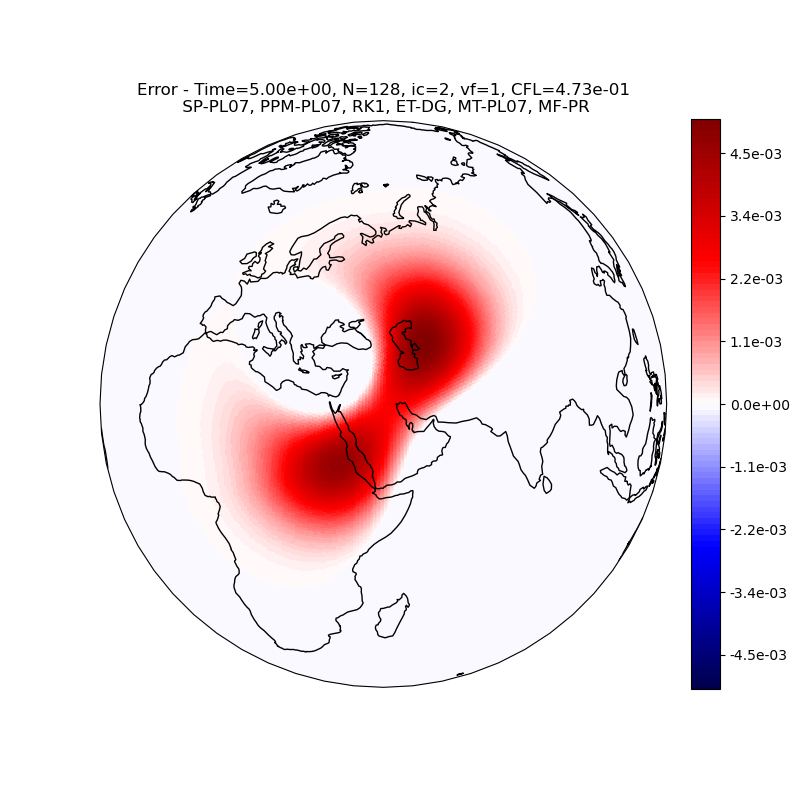
\includegraphics[width=1\linewidth]{gnomonic_equiangular_cs_128_adv_Q_error_ic2_vf1_SP-PL07_PPM-PL07_RK1_ET-DG_MT-PL07_MF-PR_interp3_t1600_sphere}
		\caption{Scheme 2 \label{chp5-adv1-s2}}
	\end{subfigure}
	
	\begin{subfigure}{0.4\textwidth}
		\centering
		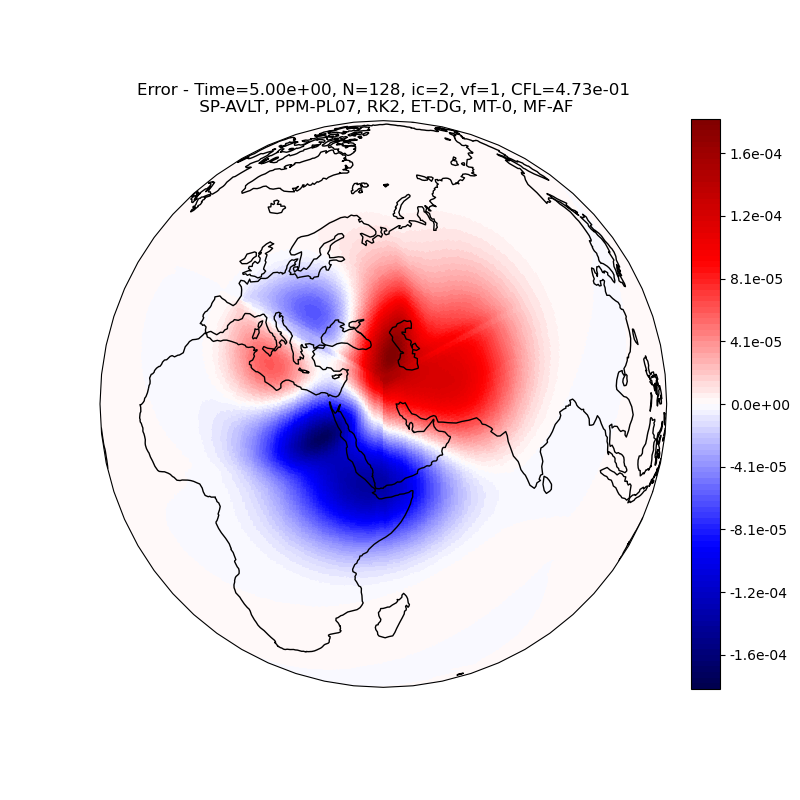
\includegraphics[width=1\linewidth]{gnomonic_equiangular_cs_128_adv_Q_error_ic2_vf1_SP-AVLT_PPM-PL07_RK2_ET-DG_MT-0_MF-AF_interp3_t1600_sphere}
		\caption{Scheme 3 \label{chp5-adv1-s3}}
	\end{subfigure}
	\begin{subfigure}{0.4\textwidth}
		\centering
		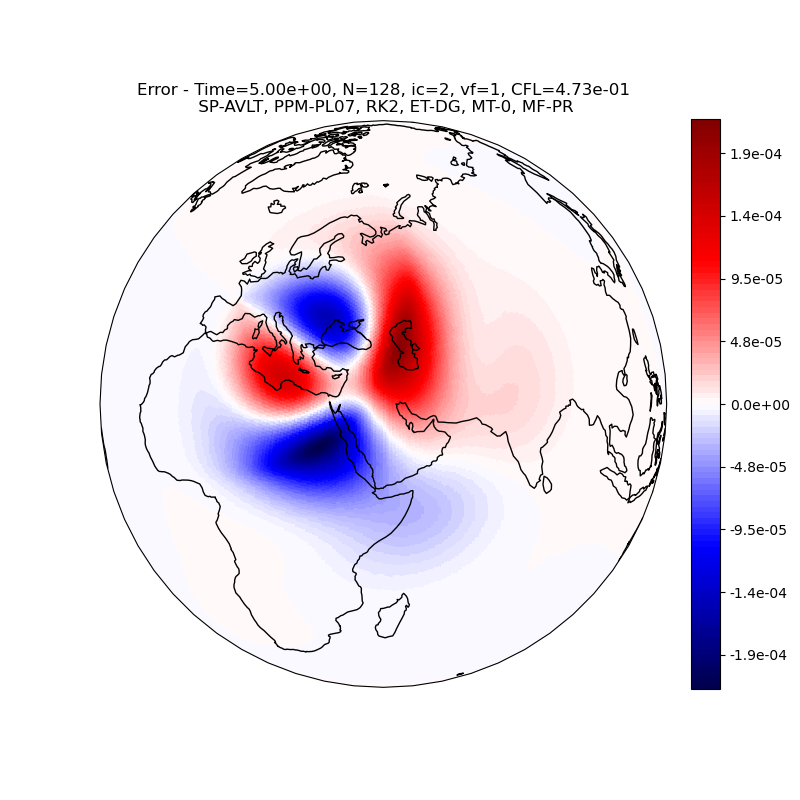
\includegraphics[width=1\linewidth]{gnomonic_equiangular_cs_128_adv_Q_error_ic2_vf1_SP-AVLT_PPM-PL07_RK2_ET-DG_MT-0_MF-PR_interp3_t1600_sphere}
		\caption{Scheme 4 \label{chp5-adv1-s4}}
	\end{subfigure}
	\caption{ Error after 5 time units obtained for all schemes from table using the VF1 velocity field from table \ref{chp5-tab2} with the initial condition IC1 from  table \ref{chp5-tab1} 
		This figure considers a cubed-sphere with $N=128$. \label{chp5-adv1}}
\end{figure}

The major difference between schemes 1 and 2 is evident from Figures \ref{chp5-adv1-s1} and
\ref{chp5-adv1-s2}, where we can observe that scheme 1 generates a grid imprinting pattern, 
while scheme 2 does not.
Similarly, scheme 3 generates grid imprinting while scheme 4 does not, 
show in Figures \ref{chp5-adv1-s3} and \ref{chp5-adv1-s4}.
We can conclude that the averaging of fluxes and the edge treatment ET-PL07 
result in more grid imprinting. However, the usage of Lagrange interpolation to fill the 
ghost cell values eliminates grid imprinting when combined with the divergence projection 
method.


\begin{figure}[!htb]
	\centering
	\begin{subfigure}{0.42\textwidth}
		\centering
		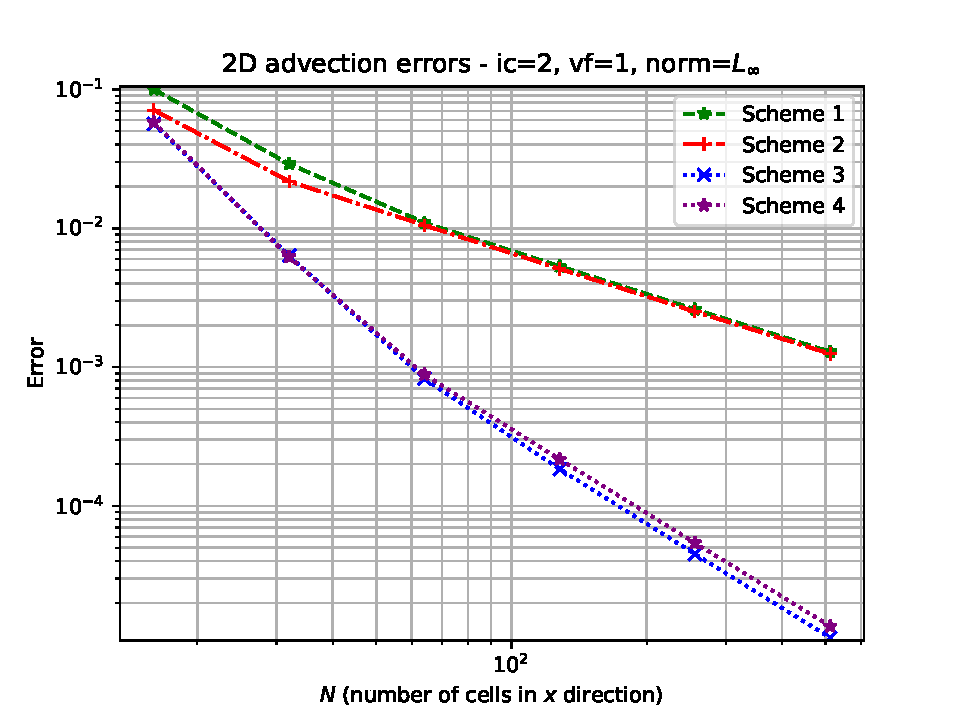
\includegraphics[width=1\linewidth]{cs_adv_tc2_ic2_vf1_normlinf_parabola_errors}
		\caption{Error.\label{chp5-adv1-error}}
	\end{subfigure}
	\begin{subfigure}{0.42\textwidth}
		\centering
		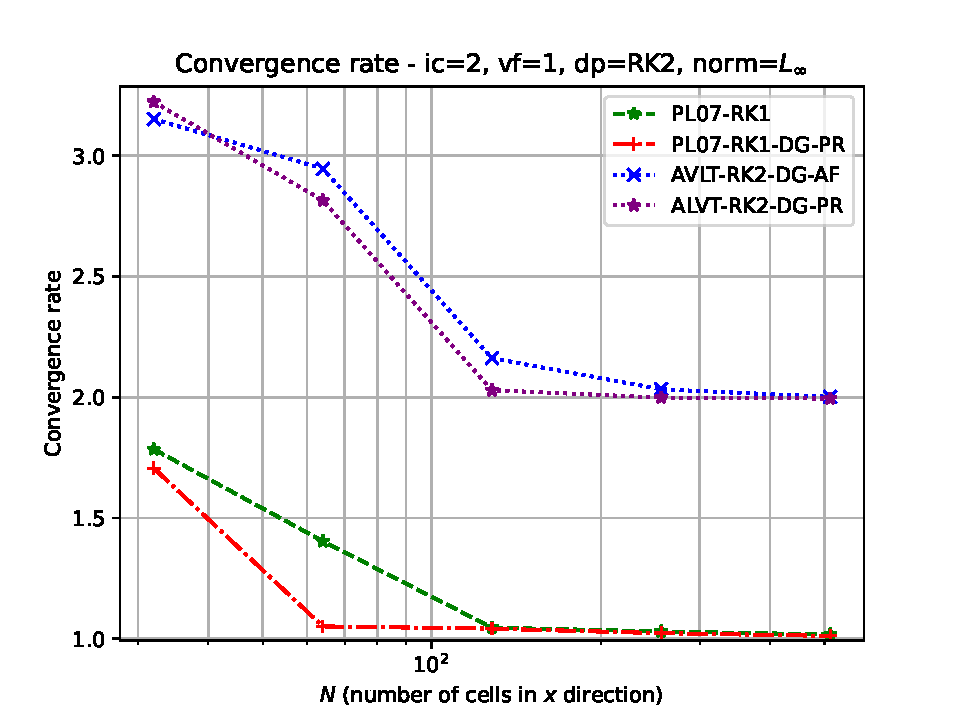
\includegraphics[width=1\linewidth]{cs_adv_tc2_ic2_vf1_normlinf_convergence_rate}
		\caption{Convergence rate.\label{chp5-adv1-cr}}
	\end{subfigure}
	\caption{Convergence of the error for the schemes from table \ref{chp5-tab3} obtained when computing the advection of IC1  with the rotated zonal wind VF1 after 5 time units.
	\label{chp5-error-adv1}}
\end{figure}



\subsection{Steady steady}
The third test case investigated focuses on IC3 with VF1. In this test, the exact solution 
remains constant and does not change over time. 
Figure \ref{chp5-error-adv1} illustrates 
the final errors obtained for all schemes listed in Table \ref{chp5-tab2}. Once again, 
schemes 1 and 2 demonstrate first-order accuracy, with scheme 2 being more accurate and 
producing no grid imprinting, as evident in Figures \ref{chp5-adv2-s1} and 
\ref{chp5-adv2-s2}. This further emphasizes the advantage of using Lagrange interpolation 
for ghost cells as opposed to the PL07 treatment.
We also observe that scheme 3 exhibits second-order accuracy, while scheme 4 demonstrates 
third-order accuracy, surpassing its expected order. However, unlike the previous test, 
scheme 4 also produces grid imprinting, although much lesser compared to scheme 3.

\begin{figure}[!htb]
	\centering
	\begin{subfigure}{0.42\textwidth}
		\centering
		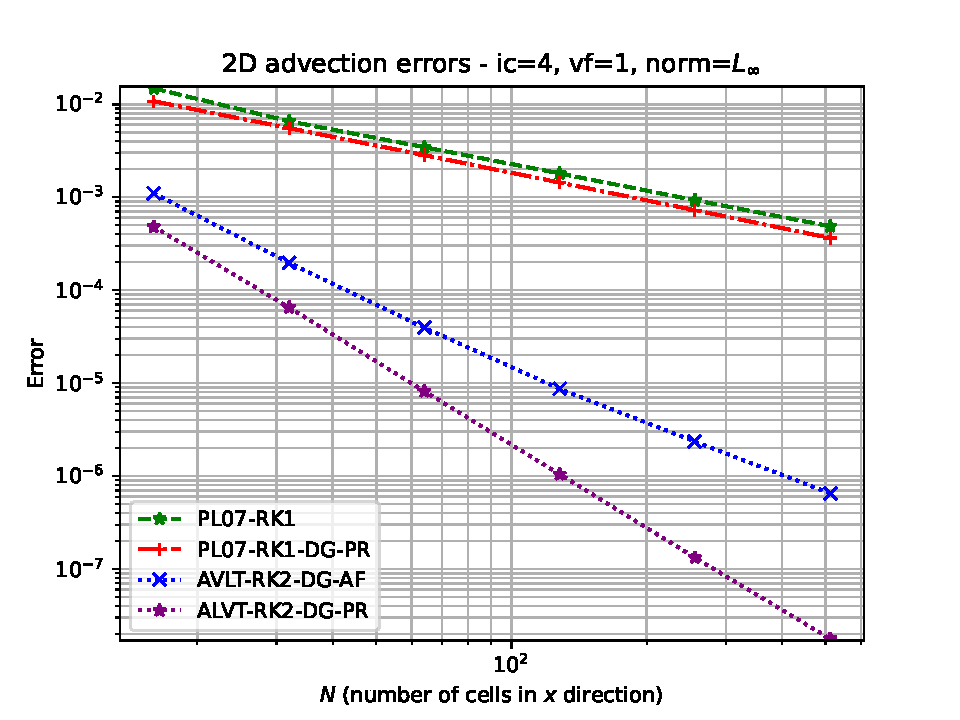
\includegraphics[width=1\linewidth]{cs_adv_tc2_ic4_vf1_normlinf_parabola_errors}
		\caption{Error.\label{chp5-adv2-error}}
	\end{subfigure}
	\begin{subfigure}{0.42\textwidth}
		\centering
		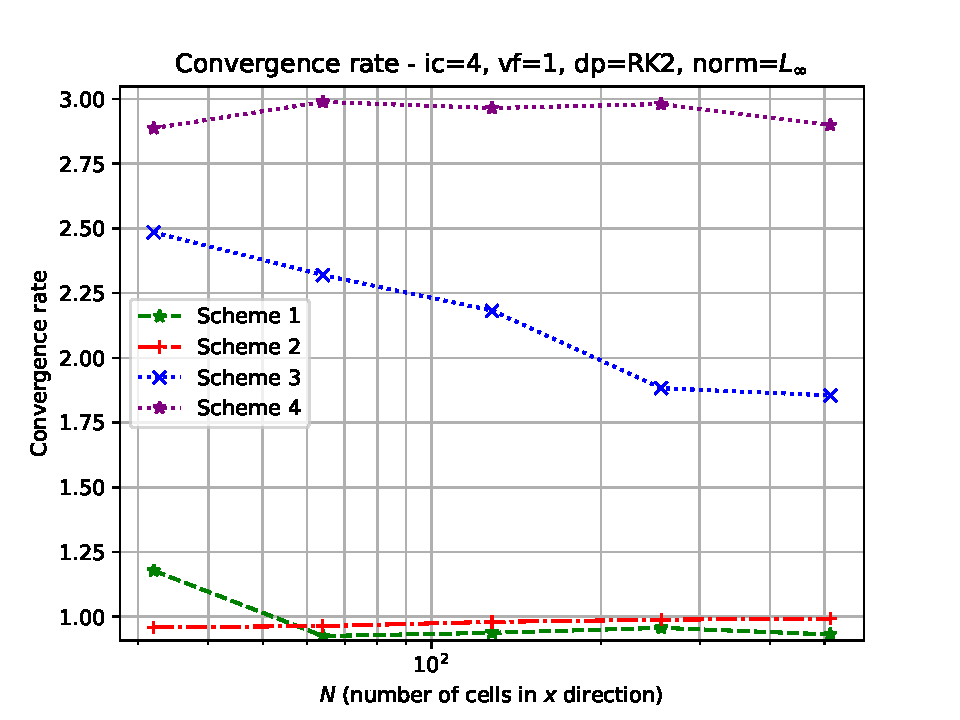
\includegraphics[width=1\linewidth]{cs_adv_tc2_ic4_vf1_normlinf_convergence_rate}
		\caption{Convergence rate.\label{chp5-adv2-cr}}
	\end{subfigure}
	\caption{Convergence of the error for the schemes from table \ref{chp5-tab3} obtained when computing the advection of IC3  with the rotated zonal wind VF1 after 5 time units.
	\label{chp5-error-adv2}}
\end{figure}


\begin{figure}[!htb]
	\centering
	\begin{subfigure}{0.3\textwidth}
		\centering
		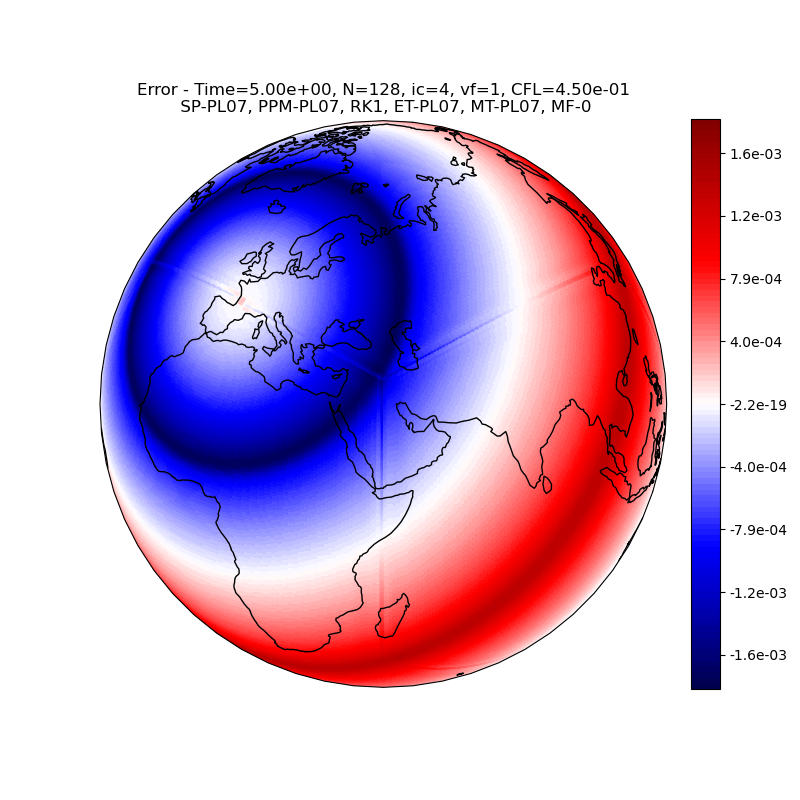
\includegraphics[width=1\linewidth]{gnomonic_equiangular_cs_128_adv_Q_error_ic4_vf1_SP-PL07_PPM-PL07_RK1_ET-PL07_MT-PL07_MF-0_interp3_t1600_sphere}
		\caption{Scheme 1 \label{chp5-adv2-s1}}
	\end{subfigure}
	\begin{subfigure}{0.3\textwidth}
		\centering
		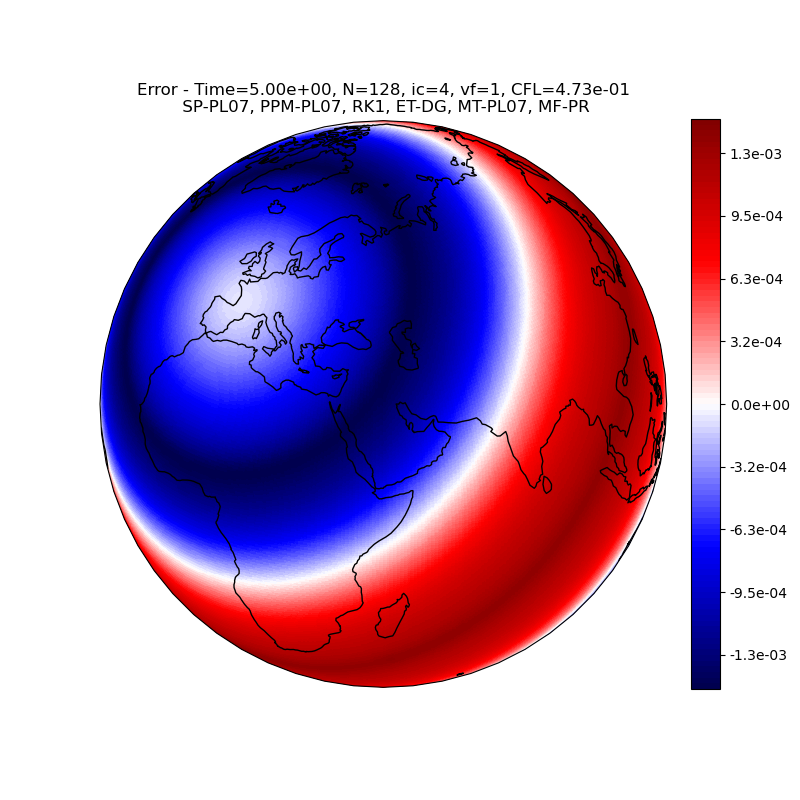
\includegraphics[width=1\linewidth]{gnomonic_equiangular_cs_128_adv_Q_error_ic4_vf1_SP-PL07_PPM-PL07_RK1_ET-DG_MT-PL07_MF-PR_interp3_t1600_sphere}
		\caption{Scheme 2 \label{chp5-adv2-s2}}
	\end{subfigure}

	\begin{subfigure}{0.3\textwidth}
		\centering
		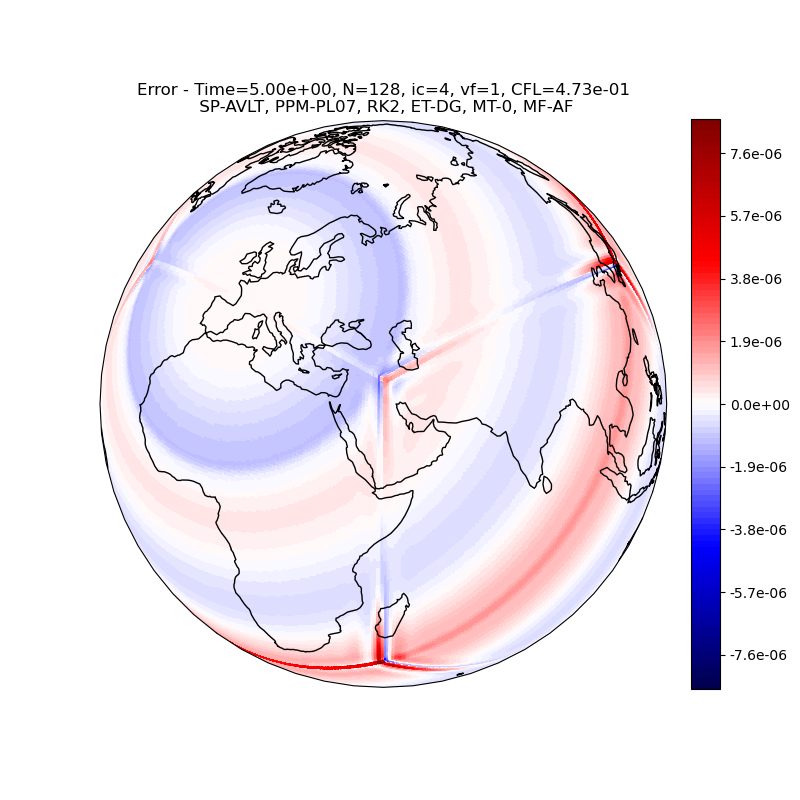
\includegraphics[width=1\linewidth]{gnomonic_equiangular_cs_128_adv_Q_error_ic4_vf1_SP-AVLT_PPM-PL07_RK2_ET-DG_MT-0_MF-AF_interp3_t1600_sphere}
		\caption{Scheme 3 \label{chp5-adv2-s3}}
	\end{subfigure}
	\begin{subfigure}{0.3\textwidth}
		\centering
		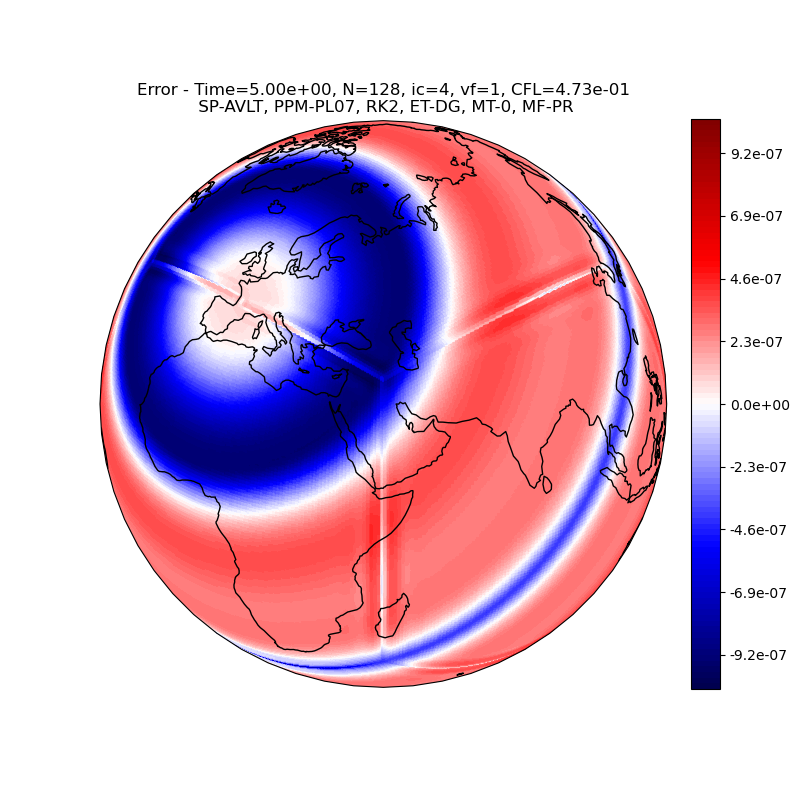
\includegraphics[width=1\linewidth]{gnomonic_equiangular_cs_128_adv_Q_error_ic4_vf1_SP-AVLT_PPM-PL07_RK2_ET-DG_MT-0_MF-PR_interp3_t1600_sphere}
		\caption{Scheme 4 \label{chp5-adv2-s4}}
	\end{subfigure}
	\caption{ Error after 5 time units obtained for all schemes from table using the VF1 velocity field from table \ref{chp5-tab2} with the initial condition IC3 from  table \ref{chp5-tab1} 
		This figure considers a cubed-sphere with $N=128$. \label{chp5-adv2}}
\end{figure}


\subsection{Non-divergent deformational flow}
As the fourth test case, we considered the non-divergent vector field VF2 velocity from table \ref{chp5-tab2}. 
We used the initial condition IC2 from table \ref{chp5-tab1}, as suggested by \citet{nair:2010}, which also shows how the solution evolves with time. 
\begin{figure}[!htb]
	\centering
	\begin{subfigure}{0.42\textwidth}
		\centering
		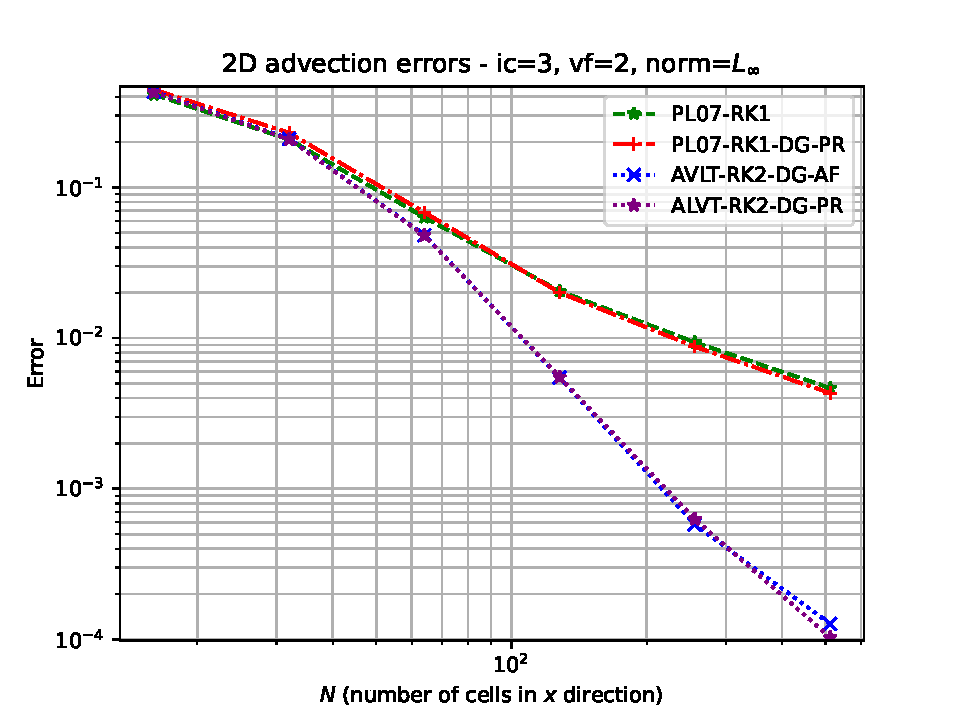
\includegraphics[width=1\linewidth]{cs_adv_tc2_ic3_vf2_normlinf_parabola_errors}
		\caption{Error.\label{chp5-adv3-error}}
	\end{subfigure}
	\begin{subfigure}{0.42\textwidth}
		\centering
		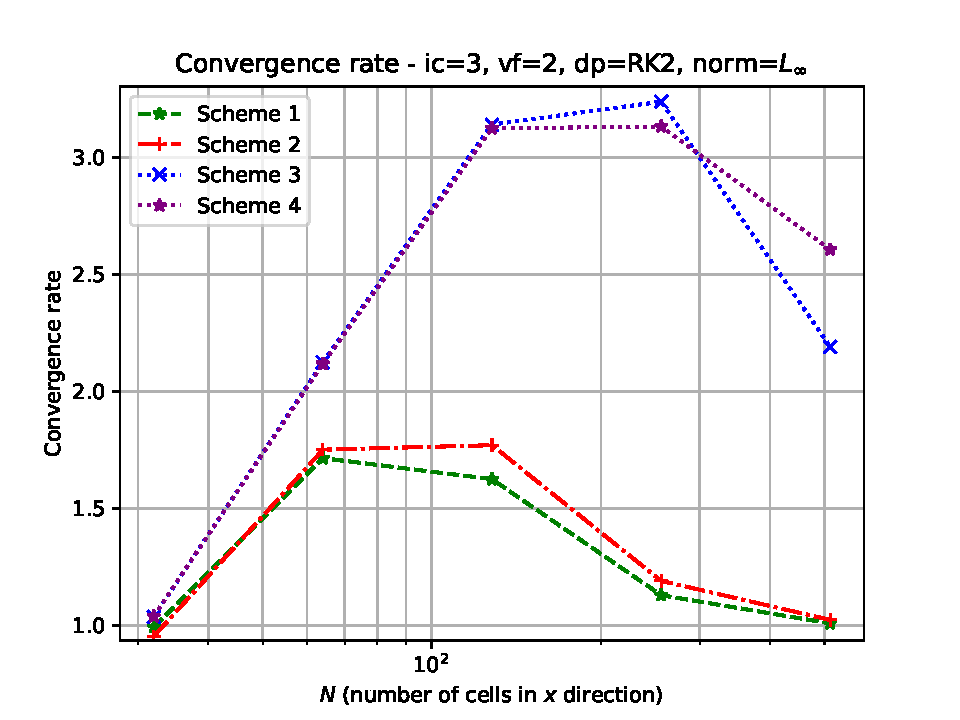
\includegraphics[width=1\linewidth]{cs_adv_tc2_ic3_vf2_normlinf_convergence_rate}
		\caption{Convergence rate.\label{chp5-adv3-cr}}
	\end{subfigure}
	\caption{Convergence of the error for the schemes from table \ref{chp5-tab3} obtained when computing the advection of IC2  with the rotated zonal wind VF3 after 5 time units.
		\label{chp5-error-adv3}}
\end{figure}

The convergence rate and errors are depicted in Figure \ref{chp5-error-adv3}.
The behavior of the error is similar to the second test.
The final errors are shown in Figure \ref{chp5-adv3}.
Unlike the previous tests, we do not observe grid-imprinting in the final errors for all the schemes.
Comparing Figure \ref{chp5-adv3-s1} with Figure \ref{chp5-adv3-s2}, we observe that the extrapolation scheme from \citet{putman:2007}
introduces numerical dispersion, which is reduced when using the duo-grid approach.
Additionally, upon comparing Figure \ref{chp5-adv3-s1} with Figure \ref{chp5-adv3-s2},
we can conclude that the divergence projection yields a smaller error than the average flux approach.
\begin{figure}[!htb]
	\centering
	\begin{subfigure}{0.35\textwidth}
		\centering
		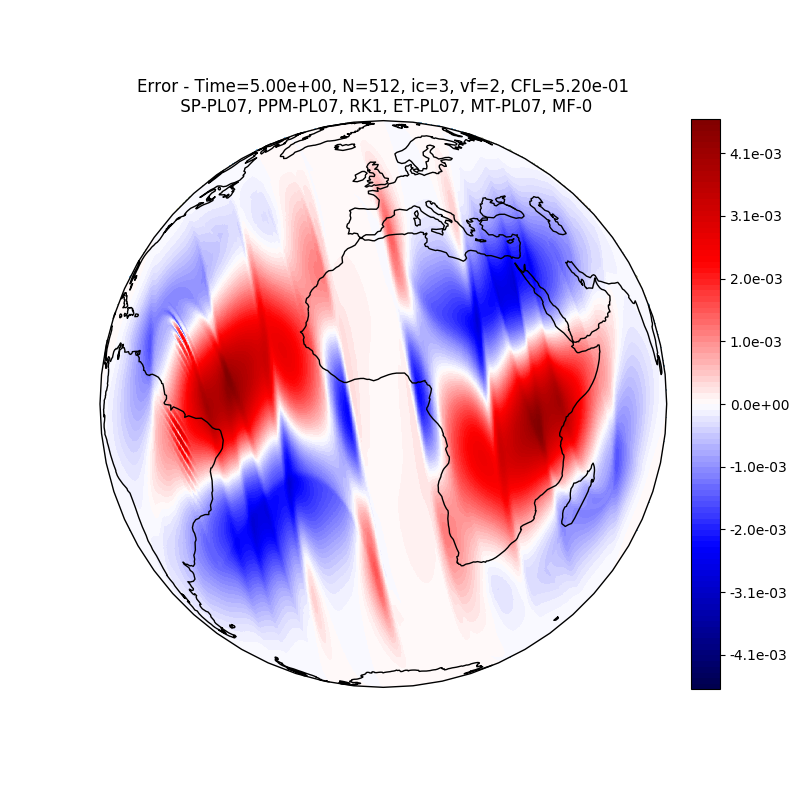
\includegraphics[width=1\linewidth]{gnomonic_equiangular_cs_512_adv_Q_error_ic3_vf2_SP-PL07_PPM-PL07_RK1_ET-PL07_MT-PL07_MF-0_interp3_t12800_sphere}
		\caption{Scheme 1 \label{chp5-adv3-s1}}
	\end{subfigure}
	\begin{subfigure}{0.35\textwidth}
		\centering
		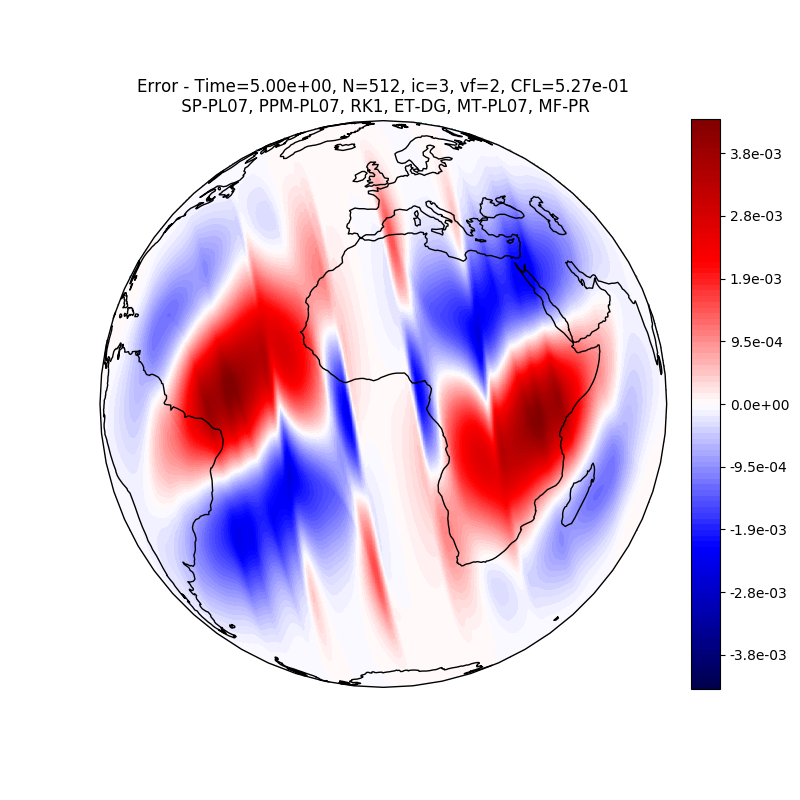
\includegraphics[width=1\linewidth]{gnomonic_equiangular_cs_512_adv_Q_error_ic3_vf2_SP-PL07_PPM-PL07_RK1_ET-DG_MT-PL07_MF-PR_interp3_t12800_sphere}
		\caption{Scheme 2 \label{chp5-adv3-s2}}
	\end{subfigure}
	
	\begin{subfigure}{0.35\textwidth}
		\centering
		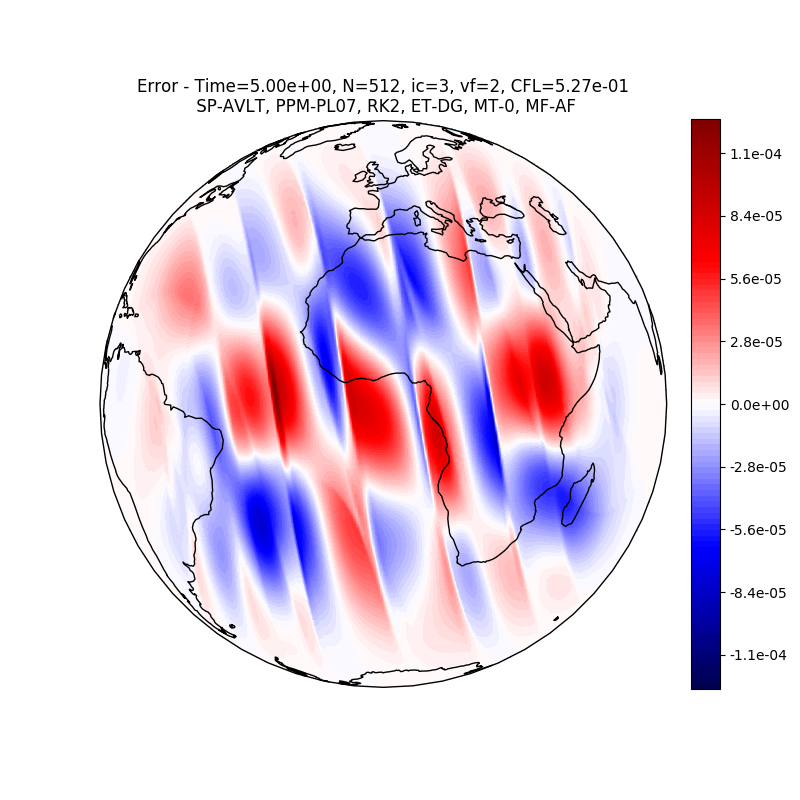
\includegraphics[width=1\linewidth]{gnomonic_equiangular_cs_512_adv_Q_error_ic3_vf2_SP-AVLT_PPM-PL07_RK2_ET-DG_MT-0_MF-AF_interp3_t12800_sphere}
		\caption{Scheme 3 \label{chp5-adv3-s3}}
	\end{subfigure}
	\begin{subfigure}{0.35\textwidth}
		\centering
		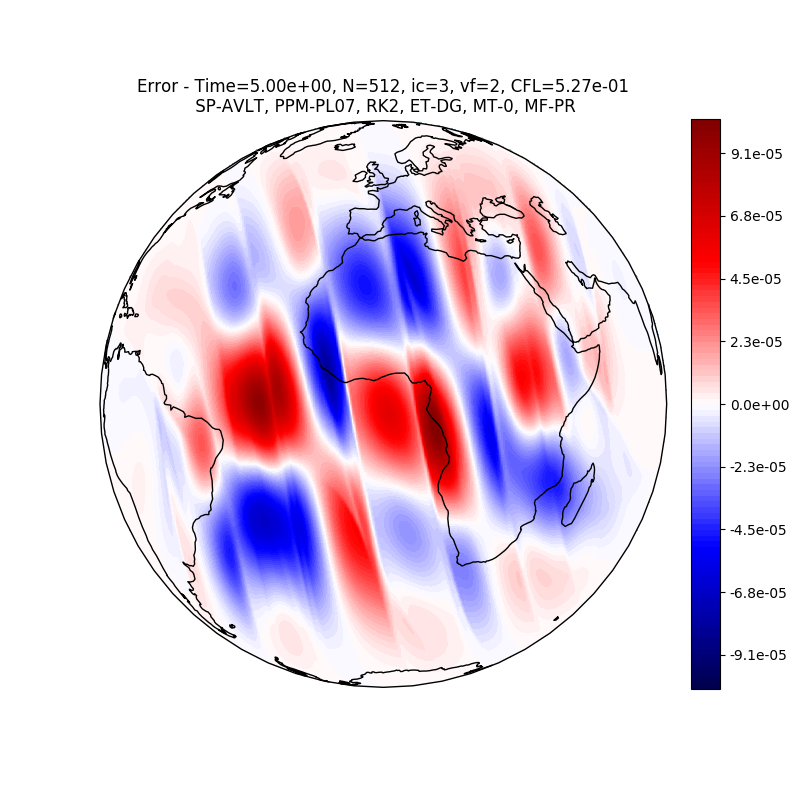
\includegraphics[width=1\linewidth]{gnomonic_equiangular_cs_512_adv_Q_error_ic3_vf2_SP-AVLT_PPM-PL07_RK2_ET-DG_MT-0_MF-PR_interp3_t12800_sphere}
		\caption{Scheme 4 \label{chp5-adv3-s4}}
	\end{subfigure}
	\caption{ Error after 5 time units obtained for all schemes from table using the VF3 velocity field from table \ref{chp5-tab2} with the initial condition IC2 from  table \ref{chp5-tab1} 
		This figure considers a cubed-sphere with $N=512$. \label{chp5-adv3}}
\end{figure}

\subsection{Divergent deformational flow}
\begin{figure}[!htb]
	\centering
	\begin{subfigure}{0.42\textwidth}
		\centering
		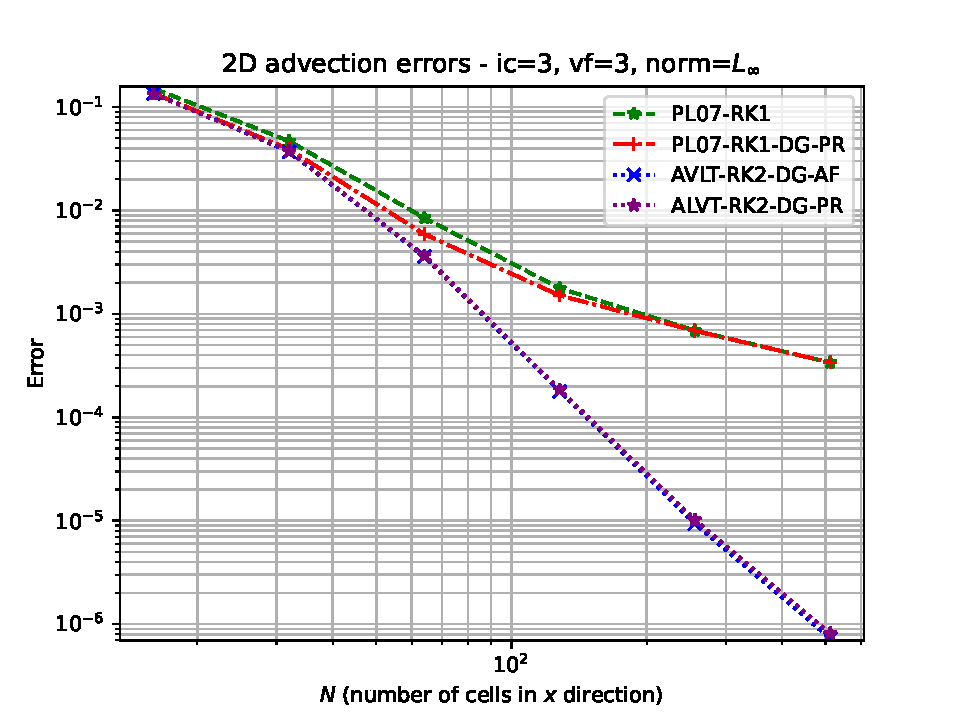
\includegraphics[width=1\linewidth]{cs_adv_tc2_ic3_vf3_normlinf_parabola_errors}
		\caption{Error.\label{chp5-adv4-error}}
	\end{subfigure}
	\begin{subfigure}{0.42\textwidth}
		\centering
		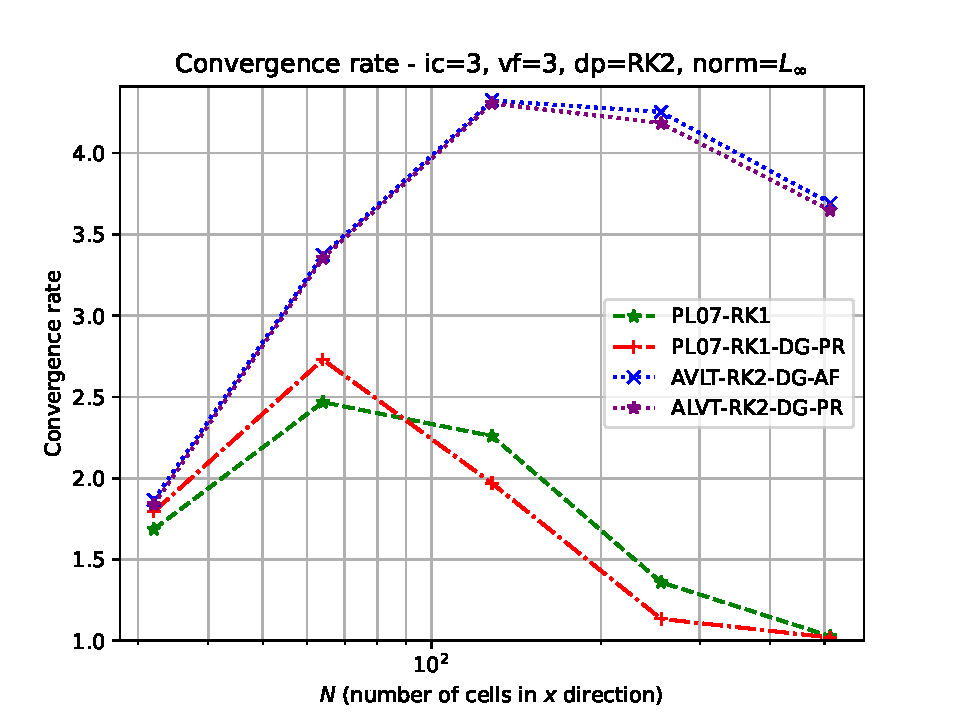
\includegraphics[width=1\linewidth]{cs_adv_tc2_ic3_vf3_normlinf_convergence_rate}
		\caption{Convergence rate.\label{chp5-adv4-cr}}
	\end{subfigure}
	\caption{Convergence of the error for the schemes from table \ref{chp5-tab3} obtained when computing the advection of IC2  with the rotated zonal wind VF3 after 5 time units.
		\label{chp5-error-adv4}}
\end{figure}


\begin{figure}[!htb]
	\centering
	\begin{subfigure}{0.35\textwidth}
		\centering
		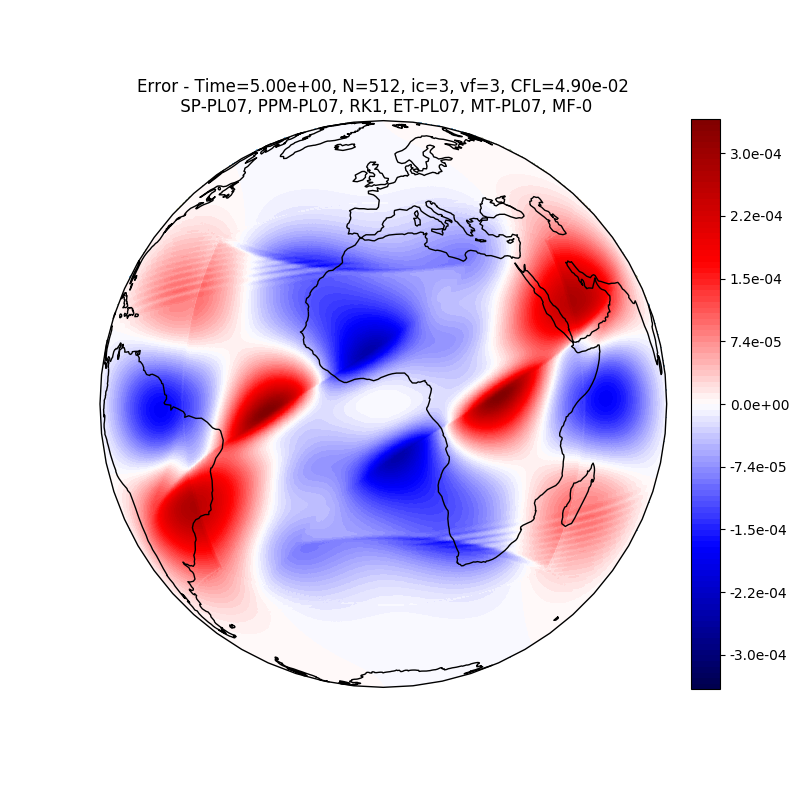
\includegraphics[width=1\linewidth]{gnomonic_equiangular_cs_512_adv_Q_error_ic3_vf3_SP-PL07_PPM-PL07_RK1_ET-PL07_MT-PL07_MF-0_interp3_t25600_sphere}
		\caption{Scheme 1 \label{chp5-adv4-s1}}
	\end{subfigure}
	\begin{subfigure}{0.35\textwidth}
		\centering
		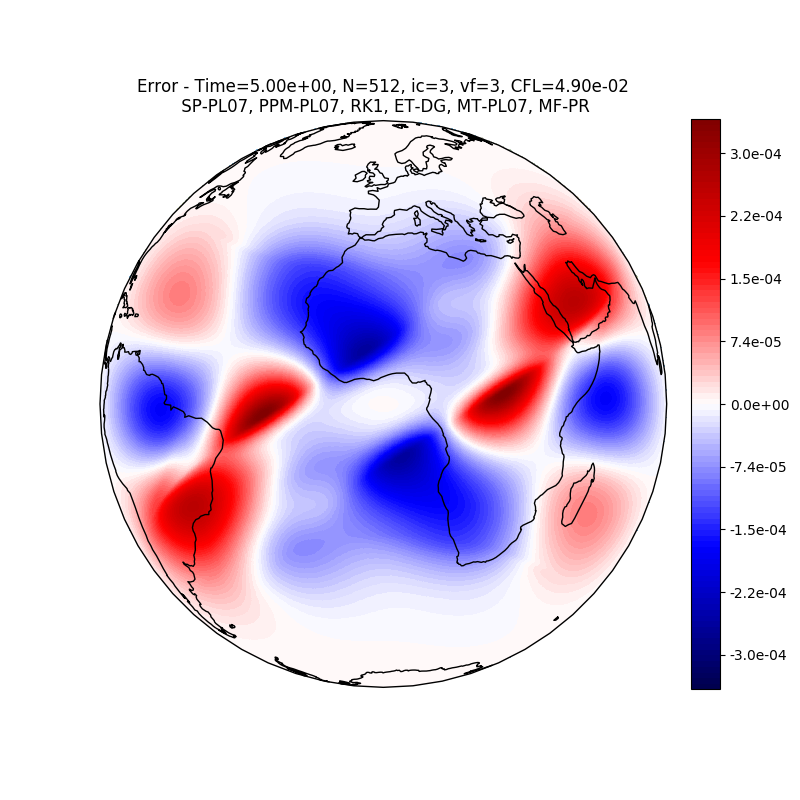
\includegraphics[width=1\linewidth]{gnomonic_equiangular_cs_512_adv_Q_error_ic3_vf3_SP-PL07_PPM-PL07_RK1_ET-DG_MT-PL07_MF-PR_interp3_t25600_sphere}
		\caption{Scheme 2 \label{chp5-adv4-s2}}
	\end{subfigure}
	
	\begin{subfigure}{0.35\textwidth}
		\centering
		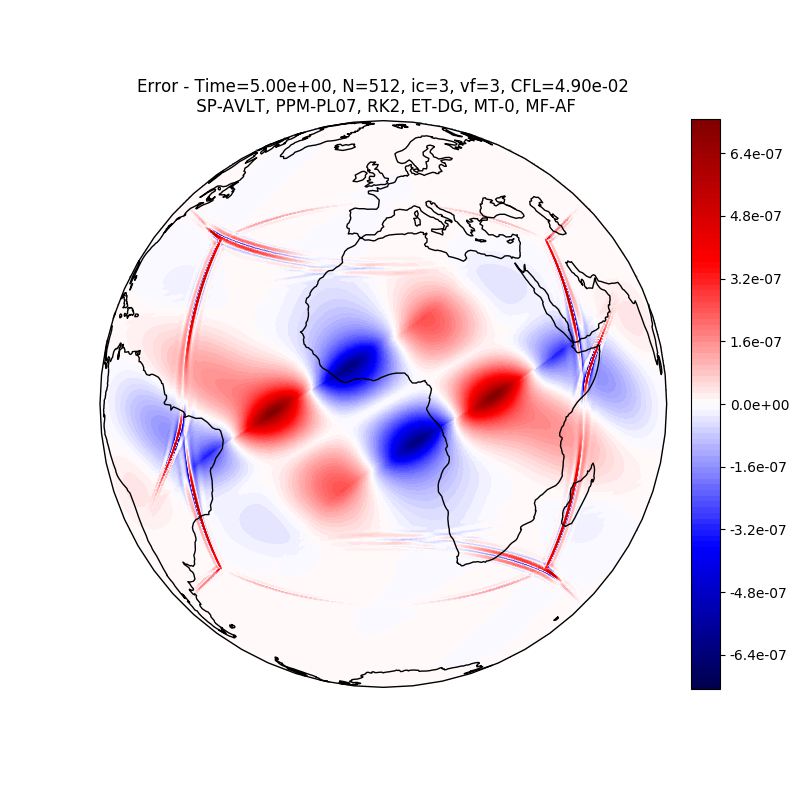
\includegraphics[width=1\linewidth]{gnomonic_equiangular_cs_512_adv_Q_error_ic3_vf3_SP-AVLT_PPM-PL07_RK2_ET-DG_MT-0_MF-AF_interp3_t25600_sphere}
		\caption{Scheme 3 \label{chp5-adv4-s3}}
	\end{subfigure}
	\begin{subfigure}{0.35\textwidth}
		\centering
		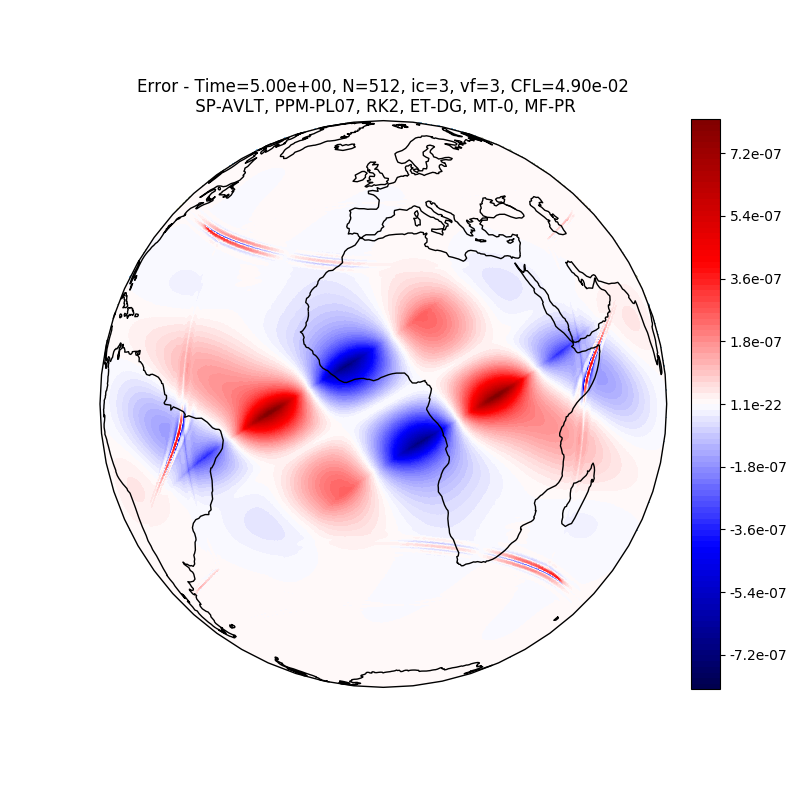
\includegraphics[width=1\linewidth]{gnomonic_equiangular_cs_512_adv_Q_error_ic3_vf3_SP-AVLT_PPM-PL07_RK2_ET-DG_MT-0_MF-PR_interp3_t25600_sphere}
		\caption{Scheme 4 \label{chp5-adv4-s4}}
	\end{subfigure}
	\caption{ Error after 5 time units obtained for all schemes from table using the VF3 velocity field from table \ref{chp5-tab2} with the initial condition IC2 from  table \ref{chp5-tab1} 
		This figure considers a cubed-sphere with $N=512$. \label{chp5-adv4}}
\end{figure}



\section{Concluding remarks}
\label{chp-cs-conc}
In this chapter, we extended the dimension splitting technique from the plane to the 
cubed-sphere. There were two essential differences in this case: 1) the presence of the 
metric tensor, and 2) the treatment of the ghost cells, which now depend on the neighboring 
panels.

Regarding the metric tensor, we explored two different approaches. One approach, as used in 
\citet{putman:2007}, involved applying the metric tensor only after integrating the PPM parabolas. 
This approach introduced a first-order error, but it facilitated the elimination of the 
splitting error for the PL07 scheme. The second approach incorporated the metric tensor in 
the PPM reconstruction and introduced no first-order error, which was crucial for achieving 
a second-order scheme.

In terms of the edge treatment schemes, we observed that the ET-PL07 scheme resulted in a 
grid-imprinting issue in the simulation. Fortunately, this grid-imprinting problem was 
resolved when we implemented the ET-DG scheme, which utilizes a third-order Lagrange 
interpolation to determine the scalar field and wind values at ghost cell positions. 
However, the main challenge with ET-DG was devising a strategy to ensure mass 
conservation at the cubed-edges.

We noticed that employing an averaging flux approach at the cube-edges led to a reduction 
in the scheme order and resulted in grid imprinting. This was as explained theoretically, where
we proved that this scheme reduces the local truncation error order by one at the cube interfaces.
As an alternative, we explored a second approach based on projecting the discrete divergence onto the space of grid 
functions with zero mass. This approach proved to be much more accurate than the averaging 
flux method.  Indeed, we showed theoretically that this approach leads to a second-order error, preserving the
accuracy of schemes that are second or first order accurate, which is our case.
However, in a steady test case, we observed that the divergence projection still caused a 
minor grid-imprinting issue.
\iffalse
\fi